\documentclass[10pt,a4paper]{article}

\usepackage[scaled]{helvet}
\usepackage[left=2.5cm,right=2.5cm,top=3cm,bottom=3cm]{geometry}
\usepackage{parskip} % don't indent first line of paragraph
\usepackage[none]{hyphenat}\sloppy  % don't hyphenate
\usepackage{tocloft}\addtolength{\cftsubsubsecnumwidth}{0.5em}\tocloftpagestyle{fancy} % fix ToC spacing issue
\usepackage{float} % [H]
\usepackage{fancyref} % \Fref
\usepackage{csquotes} % \nquote
\usepackage{enumitem} % [nolistsep]
\usepackage[printonlyused,withpage]{acronym}
\usepackage{tabularx}
\usepackage{makecell}
\usepackage[table]{xcolor}
\usepackage[hidelinks]{hyperref}\hypersetup{colorlinks, allcolors=., urlcolor=teal}
\usepackage[skins]{tcolorbox}
\usepackage{fancyhdr}
\usepackage{titling} % \thetitle, \theauthor
\usepackage{longtable}
\usepackage{array} % \arraybackslash
\usepackage{multicol}
\usepackage{textcomp} % symbols, e.g. \textdegree
\usepackage{textgreek} % greek letters, e.g. \textmu
\usepackage[super]{nth}
\usepackage{sansmath}\sansmath
\usepackage{amsmath} % bmatrix
% \usepackage{svg}
\usepackage{macros} % project specific macros
\usepackage{subcaption}
\usepackage{tablefootnote}


\renewcommand\familydefault{\sfdefault}

\graphicspath{{images/}}  % Location of the graphics files

\pagestyle{fancy}
\fancyhf{}
\fancyhead[L]{\thetitle{} \version\\ \thedate}
\fancyfoot[R]{\thepage}
\setlength{\headheight}{29pt} % must be large enough for image
\rhead{
\includegraphics[width=1.5cm]{Images/floridatech.png}}
\renewcommand{\headrulewidth}{0.5pt}
\renewcommand{\footrulewidth}{0.5pt}

\renewcommand\labelitemi{\boldmath$\cdot$} % bullet point
\renewcommand\labelitemii{-} % nested bullet point

\author{Braidan Duffy}
\title{Thetis User Manual}
\newcommand{\version}{v1.0}
\date{\today}

\begin{document}
    \begin{center}
    \vglue 2em
    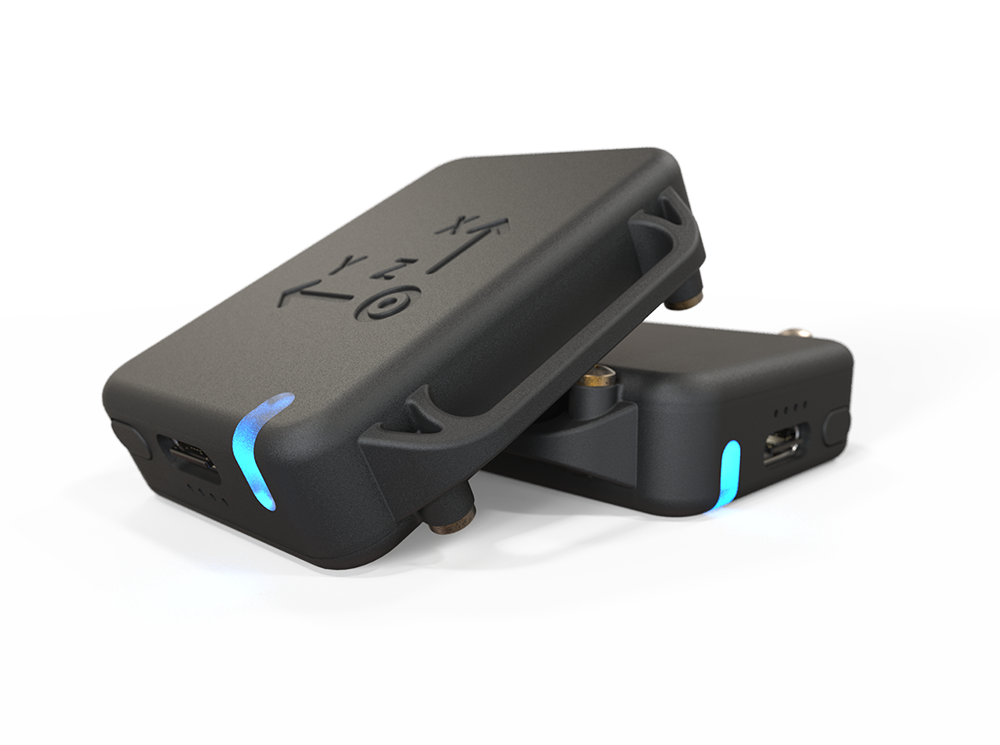
\includegraphics[width=0.8\textwidth]{Images/titlePage.png}
    \vskip 2em
    \Large\textbf{\thetitle}
    \vskip 0.5em
    \Large{\version}
    \vskip 0.5em
    \Large{\thedate}
    \vskip 1em
    \large{\theauthor}
\end{center}


    \clearpage
    \tableofcontents

    \clearpage
    \unnumberedSection{Acknowledgements}

I would like to acknowledge and thank Dr. Sebastian Madgwick, his company xio-Technologies, and his staff for their efforts in developing small embedded data loggers.
The x-IMU3 became a major inspiration when it was announced earlier in 2023 and Seb was willing to chat with me about Thetis's design and its flaws.
He has also been open to me using the x-IMU3 API on my board and the x-IMU3 user manual as a basis for this manual.
His contributions and advice directly influenced version 2.0 of the firmware and the hardware revision F6.
I am grateful for his correspondence and look forward to continuing our discussions on a variety of ideas.
    \clearpage
    \section{Overview}

\begin{multicols}{2}

The x-IMU3 is x-io Technologies' third generation \ac{IMU}.  It is a high-performance and versatile measurement device designed to accommodate a wide range of data logging and real-time applications including biomechanics, motion-capture, virtual reality, drones, robotics, and industrial.

\acs{USB}, Wi-Fi and Bluetooth provide connectivity for mobile and desktop devices while serial communication supports embedded and industrial systems.  An on-board micro \acs{SD} card allows the x-IMU3 to function as a stand-alone data logger with the ability to download files by USB and Wi-Fi.  Multiple x-IMU3s operating together on the same wireless network will automatically synchronise to stream or log synchronised measurements.

\textbf{Sensors}
\begin{itemize}[nolistsep]
    \item Gyroscope, \textpm{}2000\textdegree{}/s, 400 Hz
    \item Accelerometer, \textpm{}24 g, 400 Hz
    \item Magnetometer, \textpm{}2.5 uT, 20 Hz
    \item High-g accelerometer, \textpm{}200 g, 1600 Hz
    \item Temperature sensor\footnote{The temperature sensor is used for calibration and is not intended to provide an accurate measurement of ambient temperature.}
\end{itemize}

\textbf{Calibration}
\begin{itemize}[nolistsep]
    \item 12-parameter calibration for: axis sensitivity, axis bias, inter-axis misalignment, and package misalignment.
    \item Hard-iron and soft-iron calibration
    \item On-board gyroscope bias correction algorithm
\end{itemize}

\textbf{\acs{AHRS}}
\begin{itemize}[nolistsep]
    \item Algorithm outputs:
    \begin{itemize}
        \item Quaternion
        \item Rotation matrix
        \item Euler angles
        \item Linear acceleration
        \item Earth acceleration
    \end{itemize}
    \item Linear acceleration rejection
    \item Magnetic distortion rejection
    \item 400 Hz update rate
    \item Static accuracy:
        \begin{itemize}
            \item 1\textdegree{} \acs{RMS} inclination
            \item 2\textdegree{} \acs{RMS} heading
        \end{itemize}
\end{itemize}

\columnbreak

\textbf{Communication}
\begin{itemize}[nolistsep]
    \item \acs{USB} (\acs{CDC})
    \item Serial, 3.3V \acs{UART}
    \item \acs{TCP} (Wi-Fi)
    \item \acs{UDP} (Wi-Fi)
    \item Bluetooth (\acs{SPP})
\end{itemize}

\textbf{Wi-Fi}
\begin{itemize}[nolistsep]
    \item Client and \acs{AP} mode
    \item Dual band (2.4 GHz, 5 GHz)
    \item WPA/WPA2-Personal
    \item WPA/WPA2-Enterprise\footnote{WPA/WPA2-Enterprise security is only supported in client mode.} (TBC)
\end{itemize}

\textbf{Data logging}
\begin{itemize}[nolistsep]
    \item Supports \acs{SD} cards up to 32 GB\footnote{The product is supplied with an 8 GB \acs{SD} card that can be upgraded by the user.}
    \item Start/stop logging remotely
    \item USB download
    \item Wi-Fi download
    \item \acs{CSV} output
\end{itemize}

\textbf{Serial accessories}
\begin{itemize}[nolistsep]
    \item Receive data from external sensors and user electronics, e.g. \acs{GPS}, analogue/digital inputs, application-specific sensors.
    \item 3.3 V output to power external electronics
\end{itemize}

\textbf{Battery}
\begin{itemize}[nolistsep]
    \item Internal battery charged by \acs{USB}
    \item 15 hours data logging
    \item 11 hours Bluetooth
    \item 9 hours Wi-Fi client 2.4 GHz
    \item 6 hours Wi-Fi client 5 GHz
\end{itemize}

\textbf{Housing}
\begin{itemize}[nolistsep]
    \item IP67 (TBC)
    \item Wearable strap or chassis mount
\end{itemize}

\textbf{Software \acs{GUI}}
\begin{itemize}[nolistsep]
    \item Real-time data plots and 3D view
    \item Log real-time data to \acs{CSV}
    \item Forward real-time data to other applications
    \item Windows and OSX
\end{itemize}

\textbf{Software \acs{API}}
\begin{itemize}[nolistsep]
    \item Rust, C, C++, C\#, Python
    \item Code examples for other languages available
\end{itemize}

\end{multicols}

\clearpage

    \section{Hardware}

\subsection{Board}

Board components are annotated in \Fref{fig:board}.  A detailed mechanical drawing describing the board dimensions and locations of key components is available on the \productWebPage{}.

\vskip 2em

\begin{figure}[H]
    \centering
    \begin{tikzpicture}[annotation/.style={circle, draw=black, fill=white, very thick, minimum size=7mm}]
        \node at (0,0) {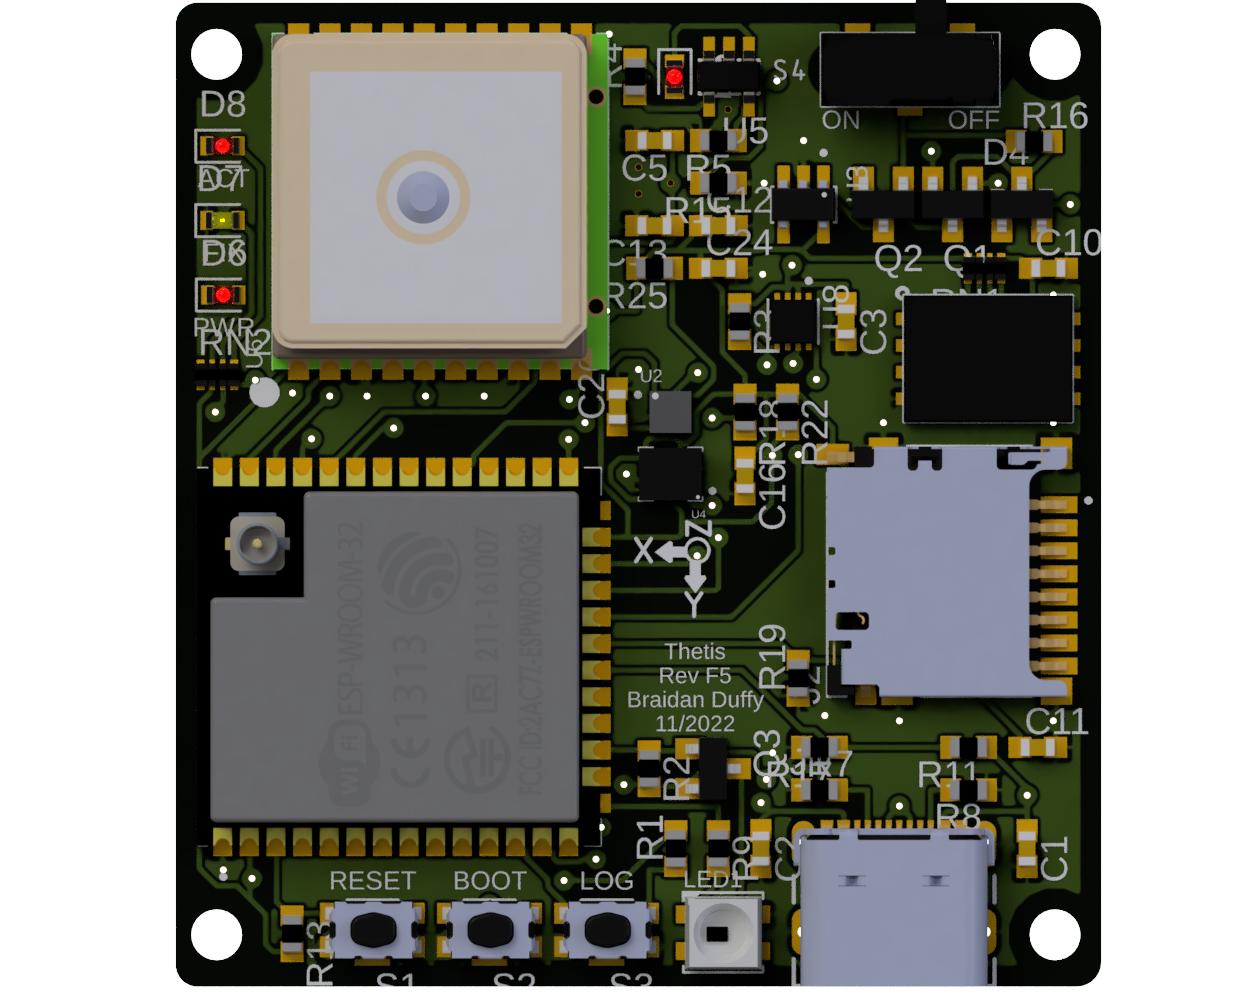
\includegraphics[width=0.95\textwidth]{Images/board.png}};
        \node[annotation] at (-6,-4) {\ref{itm:board1}};
        \node[annotation] at (-6.4,0) {\ref{itm:board2}};
        \node[annotation] at (-5.7,3.7) {\ref{itm:board3}};
        \node[annotation] at (-2.7,1.1) {\ref{itm:board4}};
        \node[annotation] at (4.8,1.8) {\ref{itm:board5}};
        \node[annotation] at (6.0,3.4) {\ref{itm:board6}};
        \node[annotation] at (7.2,3.4) {\ref{itm:board7}};
        \node[annotation] at (6.8,-1.9) {\ref{itm:board8}};
        \node[annotation] at (5.5,-4) {\ref{itm:board9}};
        \node[annotation] at (0.4,-0.8) {\ref{itm:board10}};
        \node[annotation] at (-3.4,-2.9) {\ref{itm:board11}};
    \end{tikzpicture}
    \caption{Board}
    \label{fig:board}
\end{figure}

\vskip 1em

\begin{enumerate}
    \item \label{itm:board1} Power button
    \item \label{itm:board2} \acs{USB}-C connector
    \item \label{itm:board3} \acs{LED}
    \item \label{itm:board4} Serial header
    \item \label{itm:board5} High-g accelerometer
    \item \label{itm:board6} Inertial sensor (gyroscope and accelerometer)
    \item \label{itm:board7} Magnetometer
    \item \label{itm:board8} Wireless antennae
    \item \label{itm:board9} U.FL connector for external wireless antennae
    \item \label{itm:board10} Micro \acs{SD} card socket
    \item \label{itm:board11} Battery connector
\end{enumerate}

\clearpage

\subsection{Housing}

The housing interfaces are annotated in \Fref{fig:housing}.  A detailed mechanical drawing describing the housing dimensions is available on the \productWebPage{}.

\vskip 2em

\begin{figure}[H]
    \centering
    \begin{tikzpicture}[annotation/.style={circle, draw=black, fill=white, very thick, minimum size=7mm}]
        \node at (0,0) {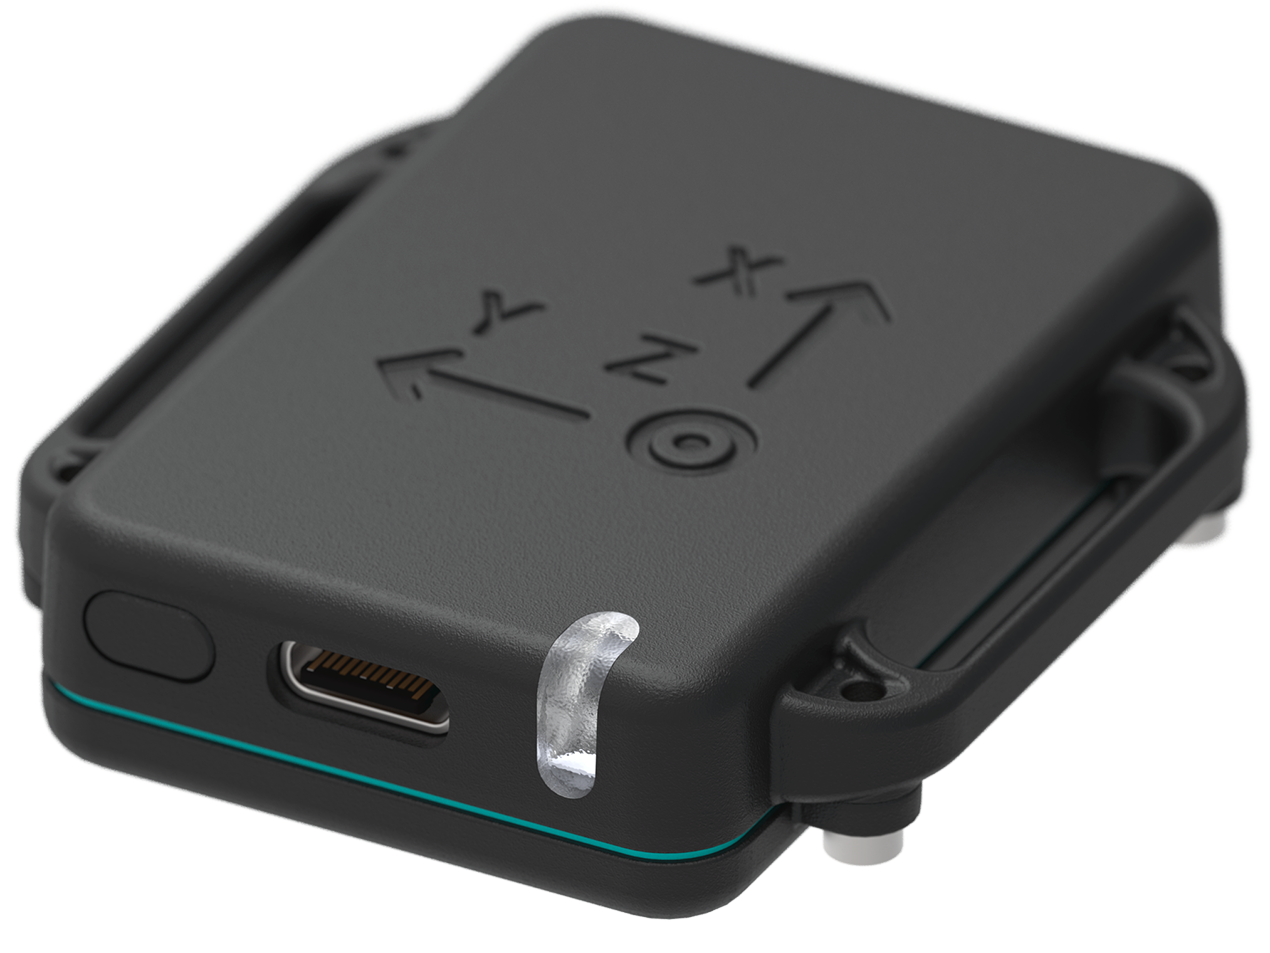
\includegraphics[width=0.8\textwidth]{Images/housing.png}};
        \node[annotation] at (-5.6,-2) {\ref{itm:housing1}};
        \node[annotation] at (-3.7,-2.55) {\ref{itm:housing2}};
        \node[annotation] at (-1.2,-3.2) {\ref{itm:housing3}};
    \end{tikzpicture}
    \caption{Housing}
    \label{fig:housing}
\end{figure}

\vskip 1em

\begin{enumerate}
    \item \label{itm:housing1} Power button
    \item \label{itm:housing2} \acs{USB}-C connector
    \item \label{itm:housing3} \acs{LED}
\end{enumerate}

\subsubsection{\acs{IP67} rating}

The \ac{IP67} rating is an international standard that describes the ability of the housing to protect against the ingress of solid particles and water.  The first digit, 6 indicates complete protection against dust and solid particles.  The second digit, 7 indicates protection from water for a maximum depth of 1 meter for up to 30 minutes.

In practical terms, this means that the housing can be used outdoors in all weather conditions and that it will survive accidental or temporary submersion in water.  The housing should \underline{not} be used in underwater applications.

% The \acs{USB}-C connector is \ac{IP67} rated and does not require a plug to...  However, the connector contains small electrical contacts that can be damaged by dirt or corrosion.  It is recommended that the \acs{USB}-C connector is protected if the housing is expected to be exposed to dust or moisture.

\clearpage

    \section{Technical Specification}

\newcommand{\techincalTable}[5]{
    \customTable
    {l c c}
    {#1 & Value & Notes}
    {
        #2
    }
    {#3}
    {#4}
    \textbf{Notes}
    \begin{enumerate}[nolistsep]
        #5
    \end{enumerate}
}

\newcommand{\characteristicTable}[4]{
    \techincalTable
    {Characteristic}
    {#1}
    {#2}
    {#3}
    {#4}
}

\newcommand{\conditionTable}[4]{
    \techincalTable
    {Condition}
    {#1}
    {#2}
    {#3}
    {#4}
}

\subsection{Mechanical}

\subsubsection{Board}

\newcommand{\noteMechanicalDrawings}[1]{A detailed mechanical drawing describing the #1 dimensions and locations of key components is available in the Appendix.}

\characteristicTable
{
    Size & 1.82 $\times$ 1.74 $\times$ 0.48 in & \ref{itm:boardMechanicalSpecification1}\\
    Weight & 3.2 g & -\\
}
{Board mechanical specification}
{tab:boardMechanicalSpecification1}
{
    \item \label{itm:boardMechanicalSpecification1} \noteMechanicalDrawings{board}
}

\characteristicTable
{
    Size & 3.15 $\times$ 2.36 $\times$ 0.79 in & \ref{itm:housingMechanicalSpecification1}\\
    Weight & 50 g & -\\
}
{Housing mechanical specification}
{tab:housingMechanicalSpecification1}
{
    \item \label{itm:housingMechanicalSpecification1} \noteMechanicalDrawings{housing}
}

\subsection{Temperature}
\label{sec:temperature}

\newcommand{\noteHeat}{The operating temperature of the device will always be greater than the surroundings due to heat generated by electronics.}

\newcommand{\noteFullRange}{The specified accuracy of the device is not achieved over the full operating temperature range.  \seeSection{sec:calibration}}

\subsubsection{No battery}

\characteristicTable
{
    Operating & -40\textdegree{}C to 85\textdegree{}C & \ref{itm:temperatureNoBattery1}, \ref{itm:temperatureNoBattery2}\\
    Storage & -40\textdegree{}C to 105\textdegree{}C & -\\
}
{Temperature specification (no battery)}
{tab:temperatureSpecificationNoBattery}
{
    \item \label{itm:temperatureNoBattery1} \noteHeat
    \item \label{itm:temperatureNoBattery2} \noteFullRange
}

\subsubsection{With battery}

\characteristicTable
{
    Operating (discharging) & -20\textdegree{}C to 60\textdegree{}C & \ref{itm:temperatureWithBattery1}, \ref{itm:temperatureWithBattery2}\\
    Operating (charging) & 0\textdegree{}C to 45\textdegree{}C & \ref{itm:temperatureWithBattery1}, \ref{itm:temperatureWithBattery2}, \ref{itm:temperatureWithBattery3}\\
    Storage & -20\textdegree{}C to 25\textdegree{}C & -\\
}
{Temperature specification (with battery)}
{tab:temperatureSpecificationWithBattery}
{
    \item \label{itm:temperatureWithBattery1} \noteHeat
    \item \label{itm:temperatureWithBattery2} \noteFullRange
    \item \label{itm:temperatureWithBattery3} Charging at temperatures below 0\textdegree{}C will reduce the capacity and cycle life of the battery.
}

\subsection{Sensors}

\newcommand{\noteRate}[1]{Each #1 includes a timestamp for a reliable measurement of time independent of the #1 rate error.  \seeSection{sec:sampleRatesMessageRatesAndTimestamps}}

\newcommand{\noteBandwidth}{The maximum bandwidth is achieved when the message rate is equal to the sample rate.  If the message rate is less than the sample rate then samples are averaged.  \seeSection{sec:sampleRatesMessageRatesAndTimestamps}}

\newcommand{\noteAccuracy}[3]{The #1 error is evaluated as the deviation of the measured magnitude of #2 for a 360\textdegree{} rotation around each axis aligned to the #3.  The magnitude is calculated as $\sqrt{x^2 + y^2 + z^2}$.}

\newcommand{\noteTemperature}{Accuracy is specified for the calibrated temperature only. \seeSection{sec:calibration}}

\subsubsection{Gyroscope}

\characteristicTable
{
    Range & \textpm{}2000\textdegree{}/s & -\\
    Resolution & 16-bit, 0.061\textdegree{}/s & -\\
    Sample rate & 100 Hz \textpm{}0.3\% & \ref{itm:gyroscope1}\\
}
{Gyroscope specification}
{tab:gyroscopeSpecification}
{
    \item \label{itm:gyroscope1} \noteRate{sample}
}

\subsubsection{Accelerometer}

\characteristicTable
{
    Range & \textpm{}32 g & -\\
    Resolution & 16-bit, 488 \textmugreek{}g & -\\
    Sample rate & 100 Hz \textpm{}0.3\% & \ref{itm:accelerometer1}\\
    Accuracy at 1 g & \textpm{}5 mg & \ref{itm:accelerometer3}, \ref{itm:accelerometer4}\\
}
{Accelerometer specification}
{tab:accelerometerSpecification}
{
    \item \label{itm:accelerometer1} \noteRate{sample}
    \item \label{itm:accelerometer3} \noteAccuracy{accelerometer}{gravity}{horizontal}
    \item \label{itm:accelerometer4} \noteTemperature
}

\subsubsection{Magnetometer}

\characteristicTable
{
    Range & \textpm{}16 Gauss & -\\
    Sample rate & 80 Hz \textpm{}8\% & \ref{itm:magnetometer1}\\
    Noise & Unknown & -\\
    Accuracy at 1 \acs{a.u.} & Unknown & \ref{itm:magnetometer2}, \ref{itm:magnetometer3}, \ref{itm:magnetometer4}\\
}
{Magnetometer specification}
{tab:magnetometerSpecification}
{
    \item \label{itm:magnetometer1} \noteRate{sample}
    \item \label{itm:magnetometer2} The calibrated magnetometer units are \ac{a.u.}.  1 \ac{a.u.} is equal to the magnitude of the ambient magnetic field during calibration, approximately 45 \textmugreek{}T.
    \item \label{itm:magnetometer3} \noteAccuracy{magnetometer}{the ambient magnetic field}{vertical}
    \item \label{itm:magnetometer4} \noteTemperature
}

\subsection{\acs{AHRS}}

\subsubsection{Update rate}

\characteristicTable
{
    Update rate & 64 Hz \textpm{}0.3\% & \ref{itm:ahrsUpdateRate1}, \ref{itm:ahrsUpdateRate2}\\
}
{\acs{AHRS} update rate}
{tab:ahrsUpdateRate}
{
    \item \label{itm:ahrsUpdateRate1} \noteRate{update}
    \item \label{itm:ahrsUpdateRate2} The \ac{AHRS} update rate is fixed independent of message rate settings.  \ac{AHRS} outputs are not averaged when the message rate is less than the update rate.
}

\subsubsection{Static accuracy}

\characteristicTable
{
    Inclination & 0.5\textdegree{} \acs{RMS} & \ref{itm:ahrsStaticAccuracy1}, \ref{itm:ahrsStaticAccuracy2}\\
    Heading & 1\textdegree{} \acs{RMS} & \ref{itm:ahrsStaticAccuracy1}, \ref{itm:ahrsStaticAccuracy2}\\
}
{\acs{AHRS} static accuracy}
{tab:ahrsStaticAccuracy}
{
    \item \label{itm:ahrsStaticAccuracy1} Static accuracy is specified as the \ac{RMS} error for a 360\textdegree{} rotation around each axis.
    \item \label{itm:ahrsStaticAccuracy2} \noteTemperature
}

\subsection{Data logger capacity}

\newcommand{\noteBinary}{The data logging capacity is specified for binary data messages.  Capacity will be reduced for \acs{ASCII} data messages.}

The data logger capacity can be determined with the following equation:

\begin{equation} \labeq{storage_time}
    t_{\text{samples}} = \frac{N_{\text{storage}} [\text{Bytes}]}{198 [\text{Bytes}] \times 64 [\text{s}^{-1}] \times 3600 \left[\frac{\text{s}}{\text{h}}\right]}
\end{equation}

This yields the following times the data logger can record for with a given \acs{microSD} card size:

\customTable
{l c}
{Size & Value}
{
    1 GB & 22 hours \\
    4 GB & 88 hours \\
    8 GB & 175 hours \\
    16 GB & 350 hours \\
    32 GB & 701 hours \\
}
{Data logger record times based on capacity of the \acs{microSD} card}
{tab:data_logger_times}

    \section{Calibration}
\label{sec:calibration}

Each device is calibrated during production to achieve the specified accuracy.  The calibration process uses specialist equipment and propriety algorithms to calculate calibration parameters specific to each device.
 Calibration is performed at room temperature.  Accuracy will be reduced for operating temperatures that deviate from this temperature.  Please refer to the calibration certificate for specific temperature values.

\subsection{Inertial sensors}
\label{sec:inertialSensor}

The inertial sensors are the gyroscope, accelerometer, and high-g accelerometer.  Each inertial sensor is calibrated for axis sensitivity, axis offset, inter-axis misalignment, and package misalignment.  The inertial calibration model is described by \Fref{eq:inertial} where $i_c$ is the calibrated inertial measurement obtained from the uncalibrated inertial measurement, $i_u$, given the misalignment matrix, $M$, the sensitivity diagonal matrix, $s$, and the offset vector, $b$.  The inertial calibration model is expanded as \Fref{eq:inertialExpanded} to express the model as 15 scalar quantities.  The units of $i_c$, $i_u$, and $b$ are degrees per second for the gyroscope, and g for the accelerometer and high-g accelerometer.  $M$ and $s$ are ratios and therefore have no units.  The calibration parameters $M$, $s$, and $b$ for each inertial sensor can be accessed as device settings.

\begin{equation}
\label{eq:inertial}
i_c = M s (i_u - b)
\end{equation}

\begin{equation}
\label{eq:inertialExpanded}
    \begin{bmatrix}
        i_{cx}\\
        i_{cy}\\
        i_{cz}\\
    \end{bmatrix}
    =
    \begin{bmatrix}
        m_{xx} & m_{xy} & m_{xz}\\
        m_{yx} & m_{yy} & m_{yz}\\
        m_{zx} & m_{zy} & m_{zz}\\
    \end{bmatrix}
    \begin{bmatrix}
        s_{x} & 0 & 0\\
        0 & s_{y} & 0\\
        0 & 0 & s_{z}\\
    \end{bmatrix}
    \left(
    \begin{bmatrix}
        i_{ux}\\
        i_{uy}\\
        i_{uz}\\
    \end{bmatrix}
    -
    \begin{bmatrix}
        b_{x}\\
        b_{y}\\
        b_{z}\\
    \end{bmatrix}
    \right)
\end{equation}

\subsection{Magnetometer}
\label{sec:magnetometer}

The magnetometer is calibrated for soft iron and hard-iron characteristics.  Soft iron characteristics are distortions that alter the intensity and direction of the magnetic field measured by the magnetometer.  Soft iron calibration also accounts for magnetometer axis sensitivity, inter-axis misalignment, and package misalignment.  Hard iron characteristics are unintended magnetic fields generated by the device that offset magnetometer measurements.  Hard iron calibration also accounts for the magnetometer axis offset.

The magnetometer calibration model is described by \Fref{eq:magnetometer} where $m_c$ is the calibrated magnetometer measurement obtained from the uncalibrated magnetometer measurement, $m_u$, given the soft iron matrix, $S$, the hard iron vector, $h$.  The magnetometer calibration model is expanded as \Fref{eq:magnetometerExpanded} to express the model as 12 scalar quantities.  The units of $m_c$, $m_u$, and $h$ are \ac{a.u.}.  $S$ is a ratio and therefore has no units.  The calibration parameters $S$, $h$ can be accessed as device settings.

\begin{equation}
\label{eq:magnetometer}
m_c = S m_u - h
\end{equation}

\begin{equation}
\label{eq:magnetometerExpanded}
    \begin{bmatrix}
        m_{cx}\\
        m_{cy}\\
        m_{cz}\\
    \end{bmatrix}
    =
    \begin{bmatrix}
        s_{xx} & s_{xy} & s_{xz}\\
        s_{yx} & s_{yy} & s_{yz}\\
        s_{zx} & s_{zy} & s_{zz}\\
    \end{bmatrix}
    \begin{bmatrix}
        m_{ux}\\
        m_{uy}\\
        m_{uz}\\
    \end{bmatrix}
    -
    \begin{bmatrix}
        h_{x}\\
        h_{y}\\
        h_{z}\\
    \end{bmatrix}
\end{equation}

\subsection{Calibration certificate}

Each device is supplied with a calibration certificate.  The calibration certificate details all calibration parameters, the calibration date, the ambient temperature and device temperature during calibration, and any equipment used during the calibration process.  The certificate also includes graphs verifying the accuracy over the measurement range.  Calibration certificates are provided as a \ac{PDF} file.  There are three ways to access the calibration certificate for a device:

\begin{enumerate}[nolistsep]
    \item Scan the \ac{QR} code on the back of the device.
    \item Open the \enquote{Calibration Certificate.html} file stored on the \ac{microSD}.
    \item Enter the device serial number on the calibration certificate \href{https://x-io.co.uk/calibration-certificate/}{web page}.
\end{enumerate}

    \section{Human Interfaces}

There are multiple human interface components on the Thetis board, as shown in \Fref{fig:revision_f5_hid}.

\begin{figure}[h!]
    \centering
    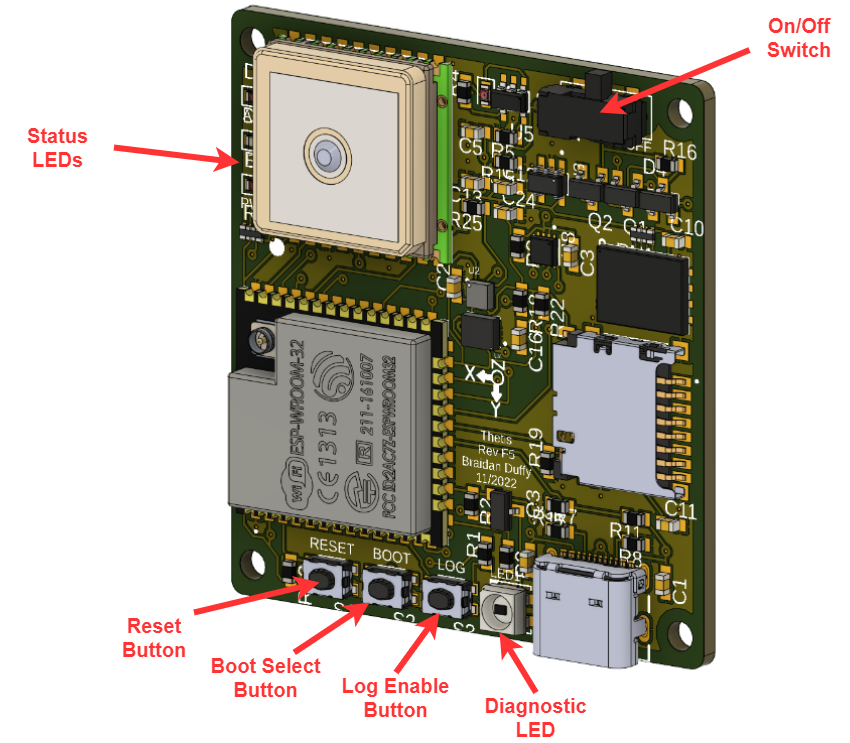
\includegraphics[height=3.5in]{revision_f5_hid.png}
    \caption{Thetis Revision F5 with callouts for human interface components}
    \labfig{revision_f5_hid}
\end{figure}

\subsection{Buttons} \label{sec:buttons}
Along the bottom edge are three buttons: reset, boot select, and log enable.

\begin{description}
    \item[The reset button] will perform a power-on reset of the microcontroller when pressed, restarting the firmware and clearing any errors.
    \item[The boot select button] will put the microcontroller into the bootloader (safe/programming) mode if pressed during a reset or power cycle. 
    \item[The log enable button] will start or stop logging when pressed for half of a second. The current logging status is shown by the LEDs. 
\end{description}

\subsection{Primary \acs{RGB} \acsp{LED}}
\label{sec:led}

The main diagnostic \ac{RGB} \ac{LED} indicates the mode and status of Thetis using different colors and flashing behaviors.

\newcommand{\ledFigure}[3]{
    \begin{figure}[H]
        \centering
        \includegraphics[width=0.5\textwidth]{LEDs/#1.png}
        \caption{#2}
        \label{fig:#3}
    \end{figure}
}

\newcommand{\ledBlinkFigure}[6]{
    \begin{figure}[H]
        \centering
        \subfloat[#2]{\includegraphics[width=0.45\textwidth]{LEDs/#1.png} \label{subfig:#6_#1}} \hskip3ex
        \subfloat[#4]{\includegraphics[width=0.45\textwidth]{LEDs/#3.png} \label{subfig:#6_#2}}
        \caption{#5}
        \label{fig:#6}
    \end{figure}
}

\subsubsection{Booting (Purple)}

A steady purple \ac{LED}, as shown in \Fref{fig:booting_led} indicates that Thetis is switched on and booting.

\ledFigure{purple}{a steady purple \acs{LED} indicating that Thetis is switched on and booting}{booting_led}

\subsubsection{Standby (Yellow)}

An steady yellow \ac{LED}, as shown in \Fref{fig:standby_led} indicates that Thetis is switched on and in standby mode. 
This mode is active until the device passes a self-test, its sensors report that they are calibrated, and the fusion algorithm is online and stable.
Currently, this mode is bypassed and ignored.

\ledFigure{yellow}{A steady yellow \acs{LED} indicating that Thetis is switched on and in standby mode}{standby_led}

\subsubsection{Ready, No GPS (Blue)}

A blinking (once per second) blue \ac{LED}, as shown in \Fref{fig:ready_no_gps_led} indicates that Thetis is online, calibrated, and ready to start logging.
However, it has not yet acquired a GPS fix.
This mode will still allow logging, but the position messages will either not be populated or not accurate.

% \ledBlinkFigure{blue}{The \ac{LED} is blue for approximately 1 second}{off}{Then turns off for one second}{A blinking blue \ac{LED} indicating that Thetis is switched on and ready to log data without a GPS fix}{ready_no_gps_led}

\begin{figure}[H]
    \centering
    \subfloat[The \ac{LED} is blue for approximately 250 milliseconds]{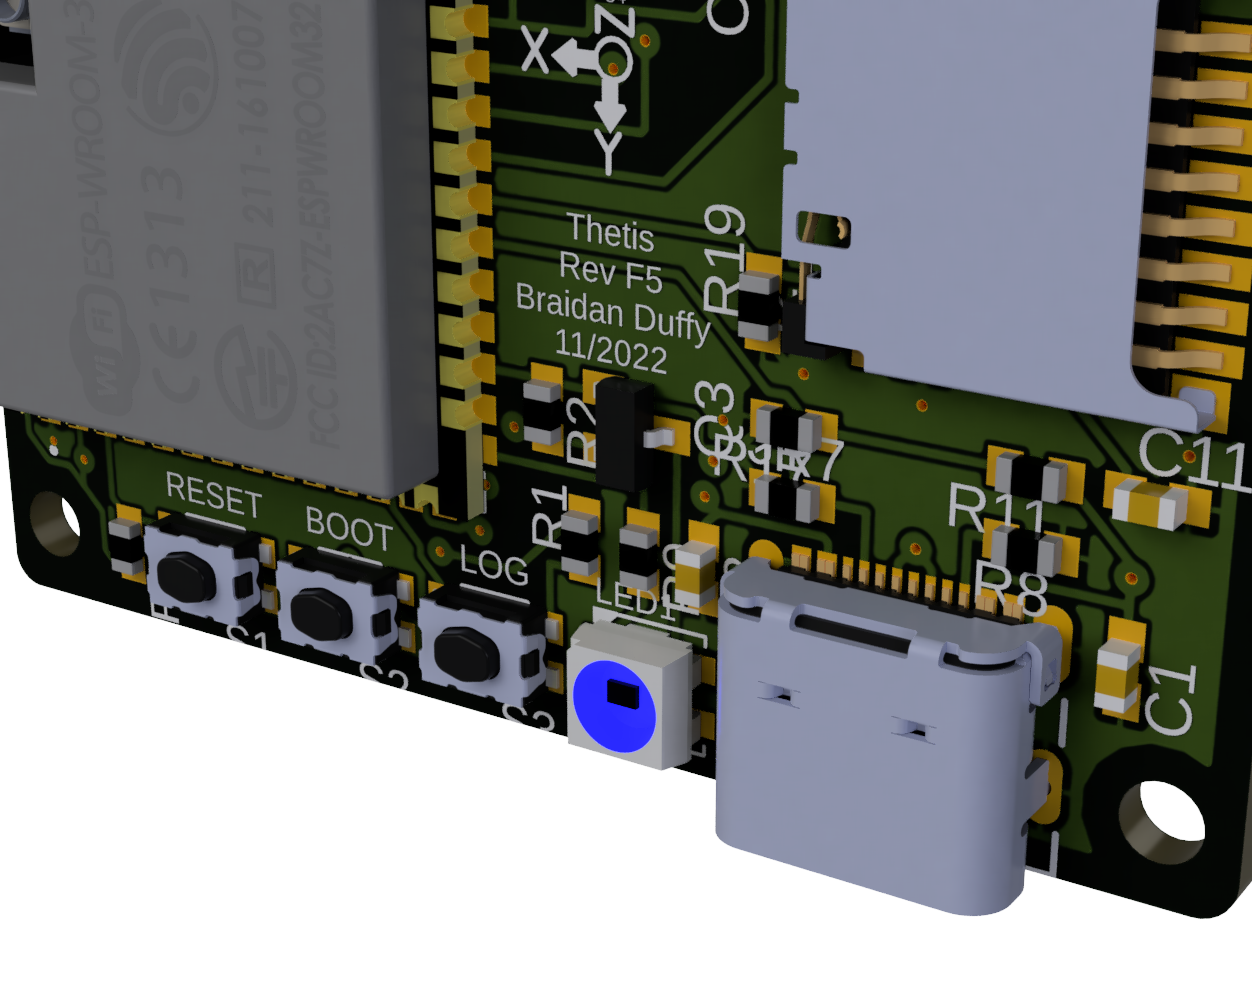
\includegraphics[width=0.45\textwidth]{LEDs/blue.png} \label{subfig:ready_no_gps_led_blue}} \hskip3ex
    \subfloat[Then turns off for 250 milliseconds]{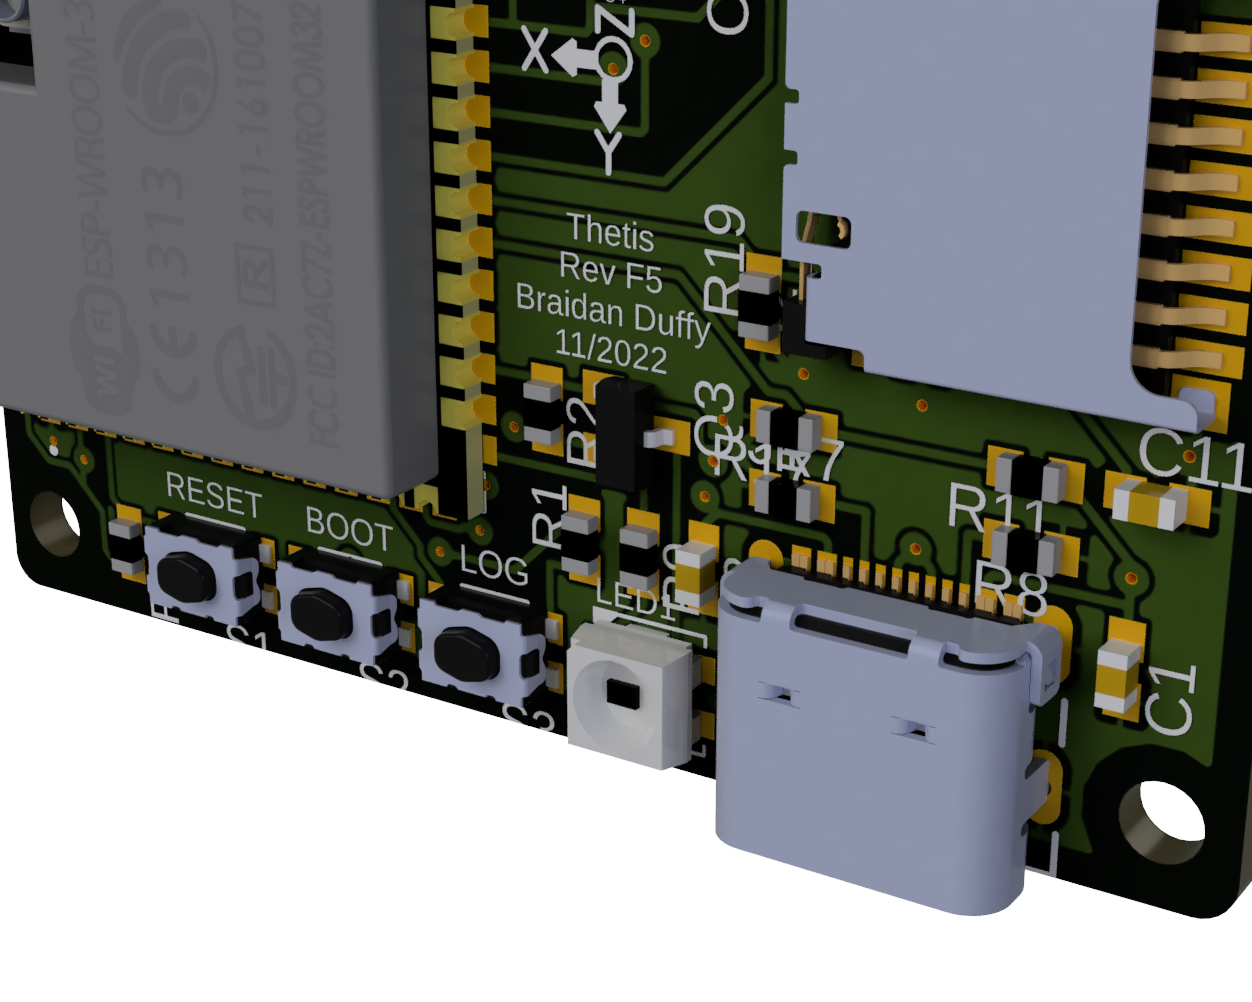
\includegraphics[width=0.45\textwidth]{LEDs/off.png} \label{subfig:ready_no_gps_led_off}}
    \caption{A blinking blue \ac{LED} indicating that Thetis is switched on and ready to log data without a GPS fix}
    \label{fig:ready_no_gps_led}
\end{figure}

\subsubsection{Logging, No GPS (Blue)}

A steady blue \ac{LED}, as shown in \Fref{fig:logging_no_gps_led} indicates that Thetis is switched on and logging data without a GPS fix.
This mode will still log data as expected, but the position messages will either not be populated or not accurate.

\ledFigure{blue}{A steady blue \acs{LED} indicating that Thetis is switched on and logging without a GPS fix}{logging_no_gps_led}

\subsubsection{Ready, GPS (Green)}

A blinking (once per second) green \ac{LED}, as shown in \Fref{fig:ready_gps_led} indicates that Thetis is online, calibrated, and ready to start logging with a valid GPS fix.
This will populate the position message with reasonably-accurate GPS data.

% \ledFigure{ready_gps_led}{A blinking green \acs{LED} indicating that Thetis is switched on and ready to log data with a GPS fix}

\begin{figure}[H]
    \centering
    \subfloat[The \ac{LED} is green for 250 milliseconds]{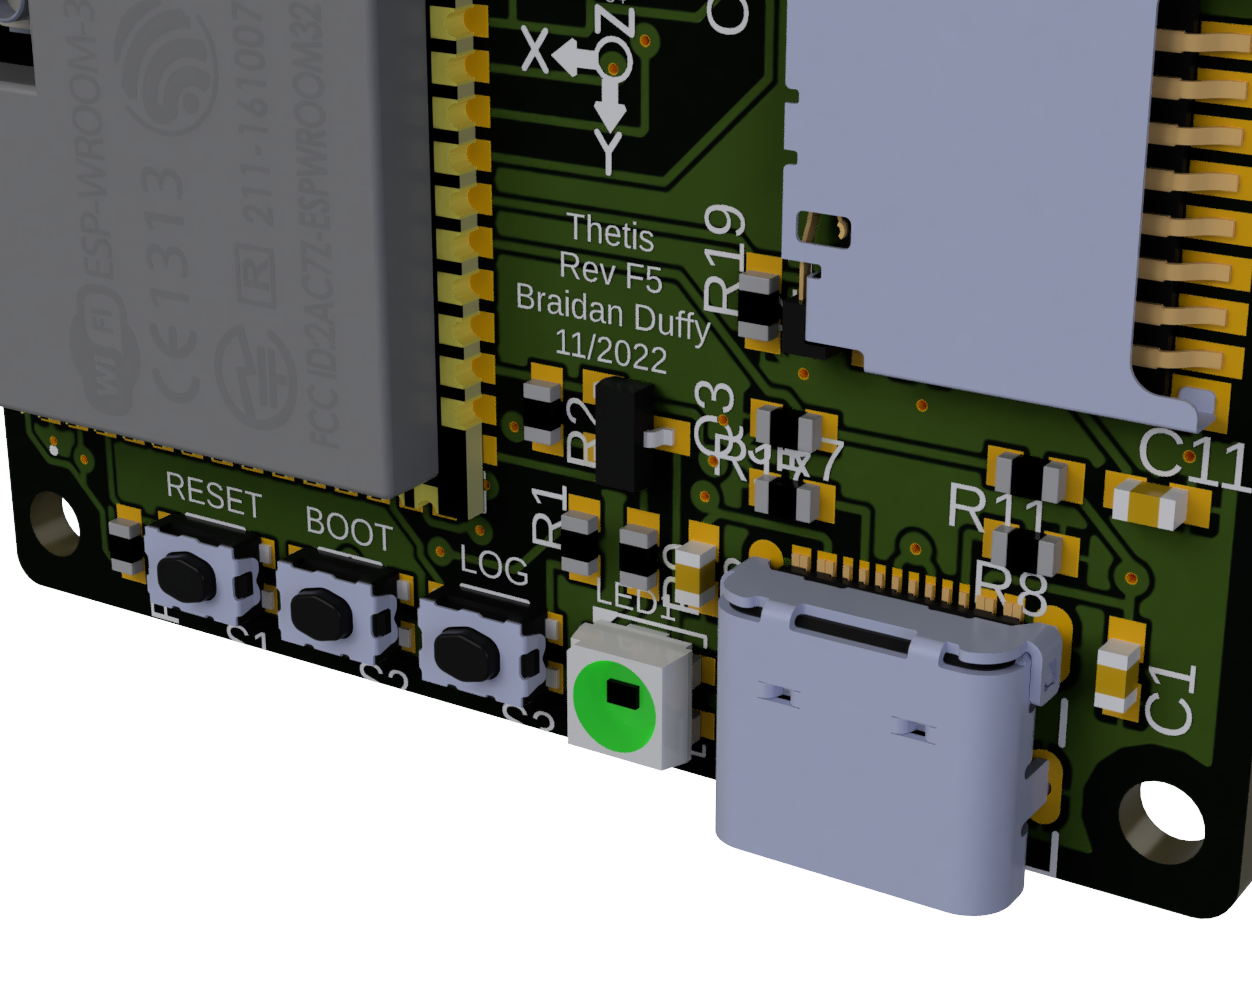
\includegraphics[width=0.45\textwidth]{LEDs/green.png} \label{subfig:ready_gps_led_green}} \hskip3ex
    \subfloat[Then turns off for 250 milliseconds]{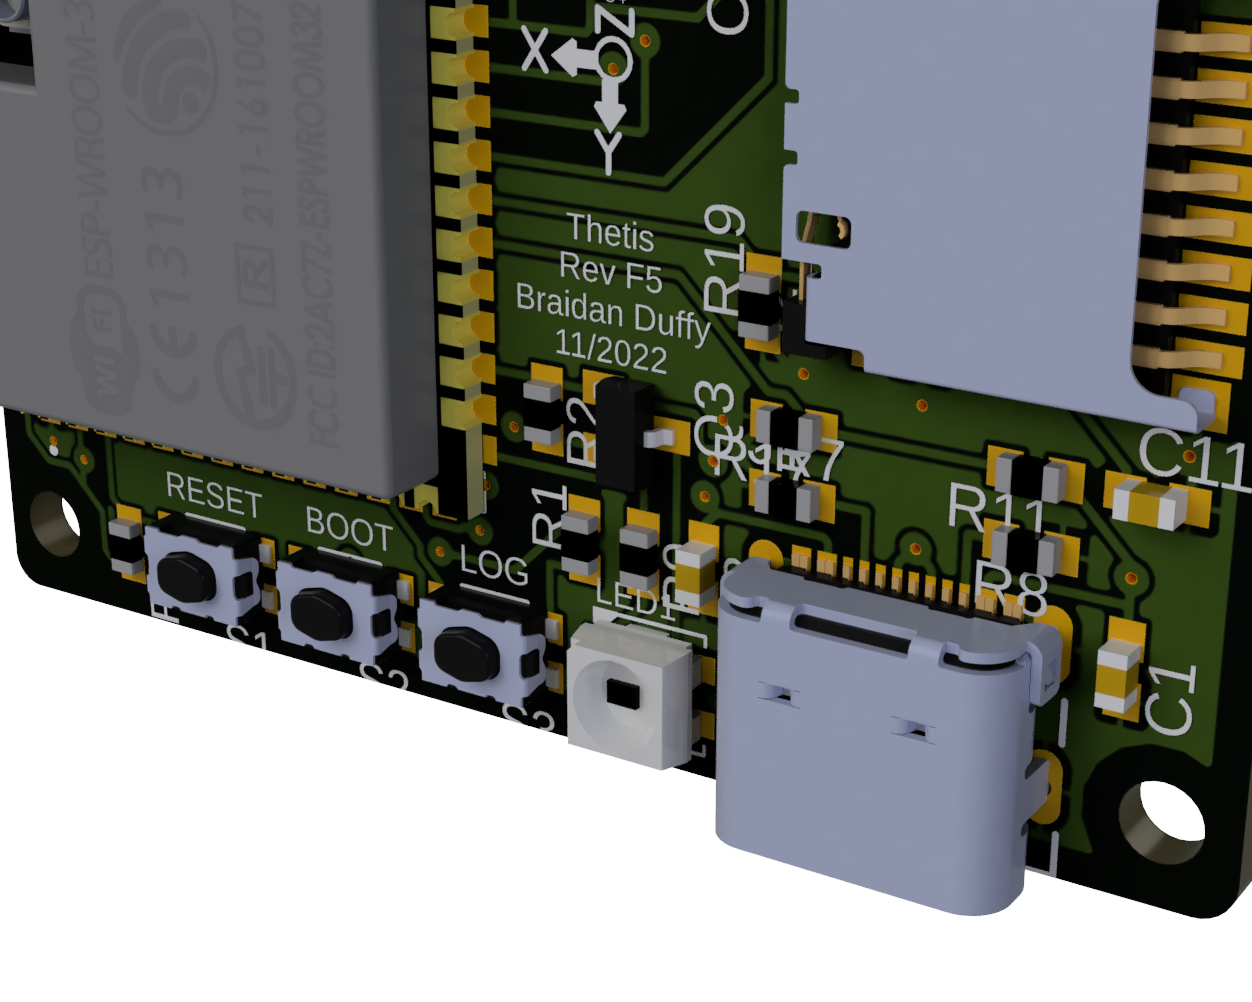
\includegraphics[width=0.45\textwidth]{LEDs/off.png} \label{subfig:ready_gps_led_off}}
    \caption{A blinking green \ac{LED} indicating that Thetis is switched on and ready to log data with a GPS fix}
    \label{fig:ready_gps_led}
\end{figure}

\subsubsection{Logging, GPS (Green)}

A steady green \ac{LED}, as shown in \Fref{fig:logging_gps_led} indicates that Thetis is switched on and logging data with a GPS fix.
Position messages will be populated with reasonably-accurate GPS data in this mode.

\ledFigure{green}{A steady green \acs{LED} indicating that Thetis is switched on and logging with a GPS fix}{logging_gps_led}

\subsubsection{Error (Red and Yellow)}

When Thetis enters an error state, the main \acs{RGB} \ac{LED} will begin flashing red and yellow error codes based on the error type.
The red blinks will precede the yellow blinks and there will be a short interval between code flashes.
In the error state, Thetis will lock up and lose all functionality until the battery dies.
The device will require a full power cycle or reset to clear the error code.
In-depth diagnostic information may be available if data is being streamed to a host computer through the USB port and serial monitor terminal (e.g. PuTTY).

\begin{figure}[H]
    \centering
    \subfloat[The \ac{LED} is red with 250 millisecond blinks for a certain number of times]{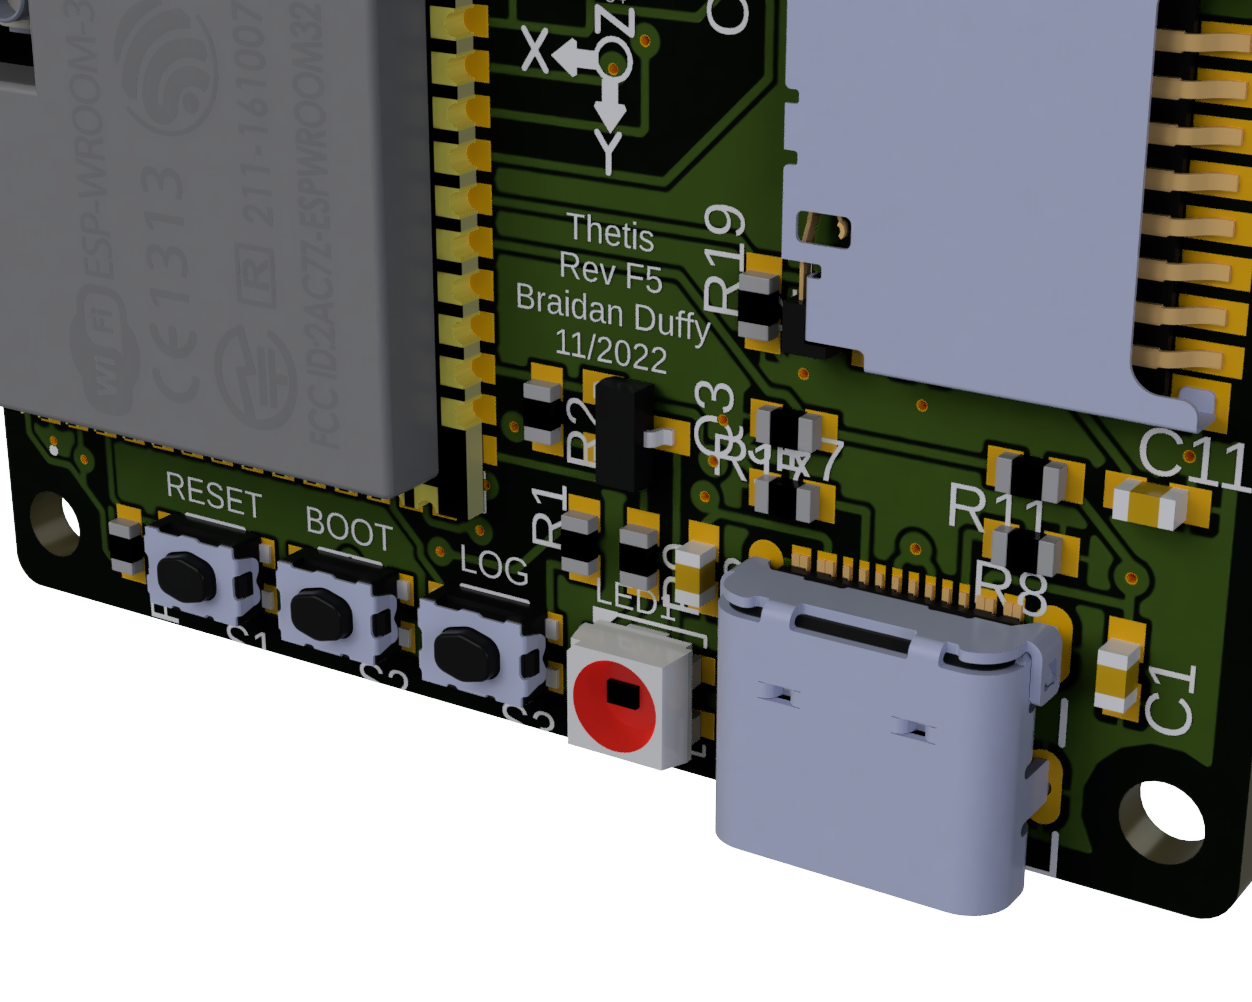
\includegraphics[width=0.3\textwidth]{LEDs/red.png} \label{subfig:error_green}} \hskip3ex
    \subfloat[Then turns yellow with 250 millisecond blinks for a certain number of times]{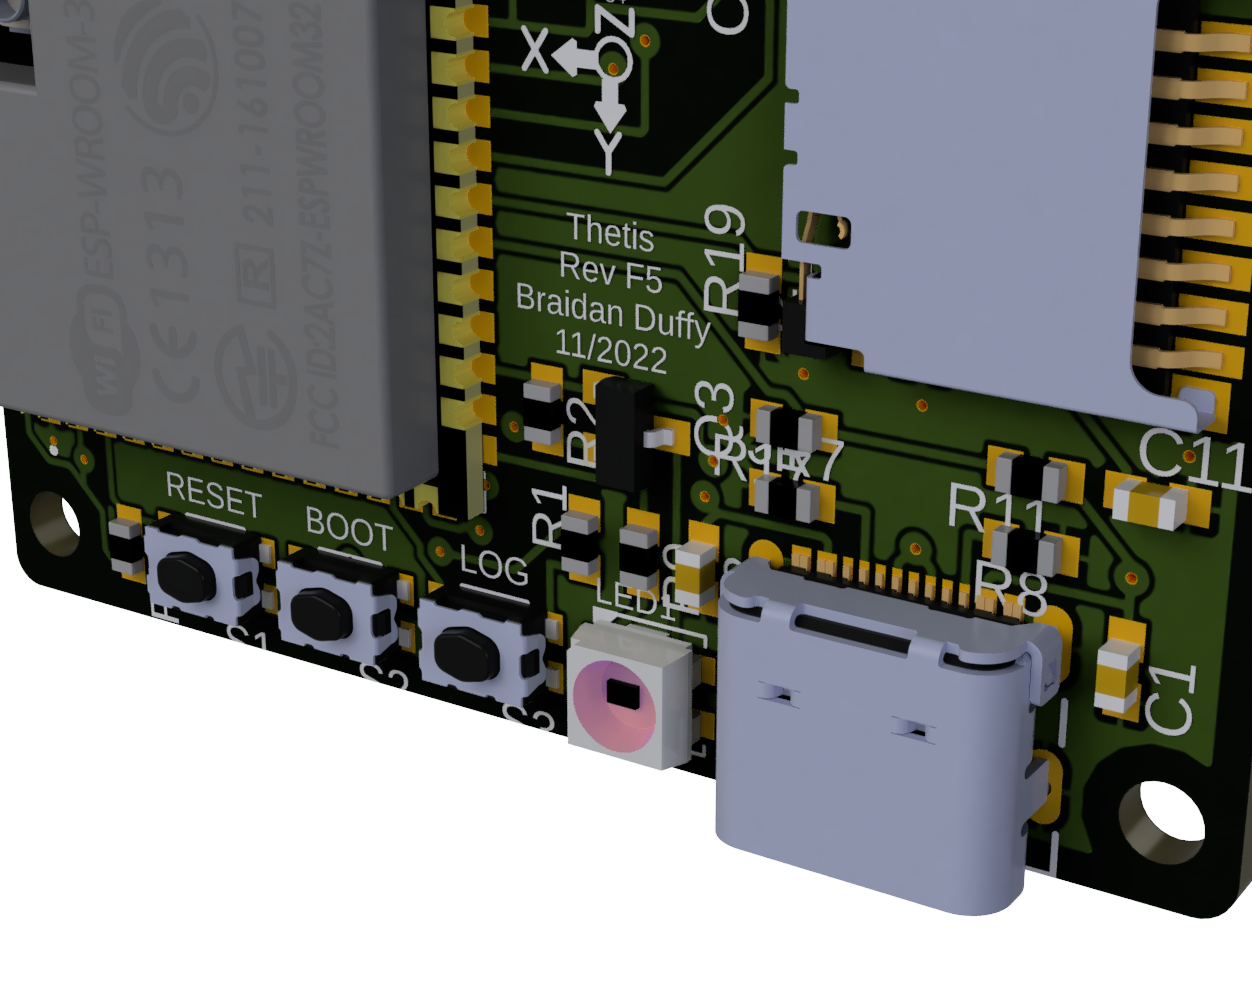
\includegraphics[width=0.3\textwidth]{LEDs/yellow.png} \label{subfig:error_yellow}} \hskip3ex
    \subfloat[Then turns off for one second]{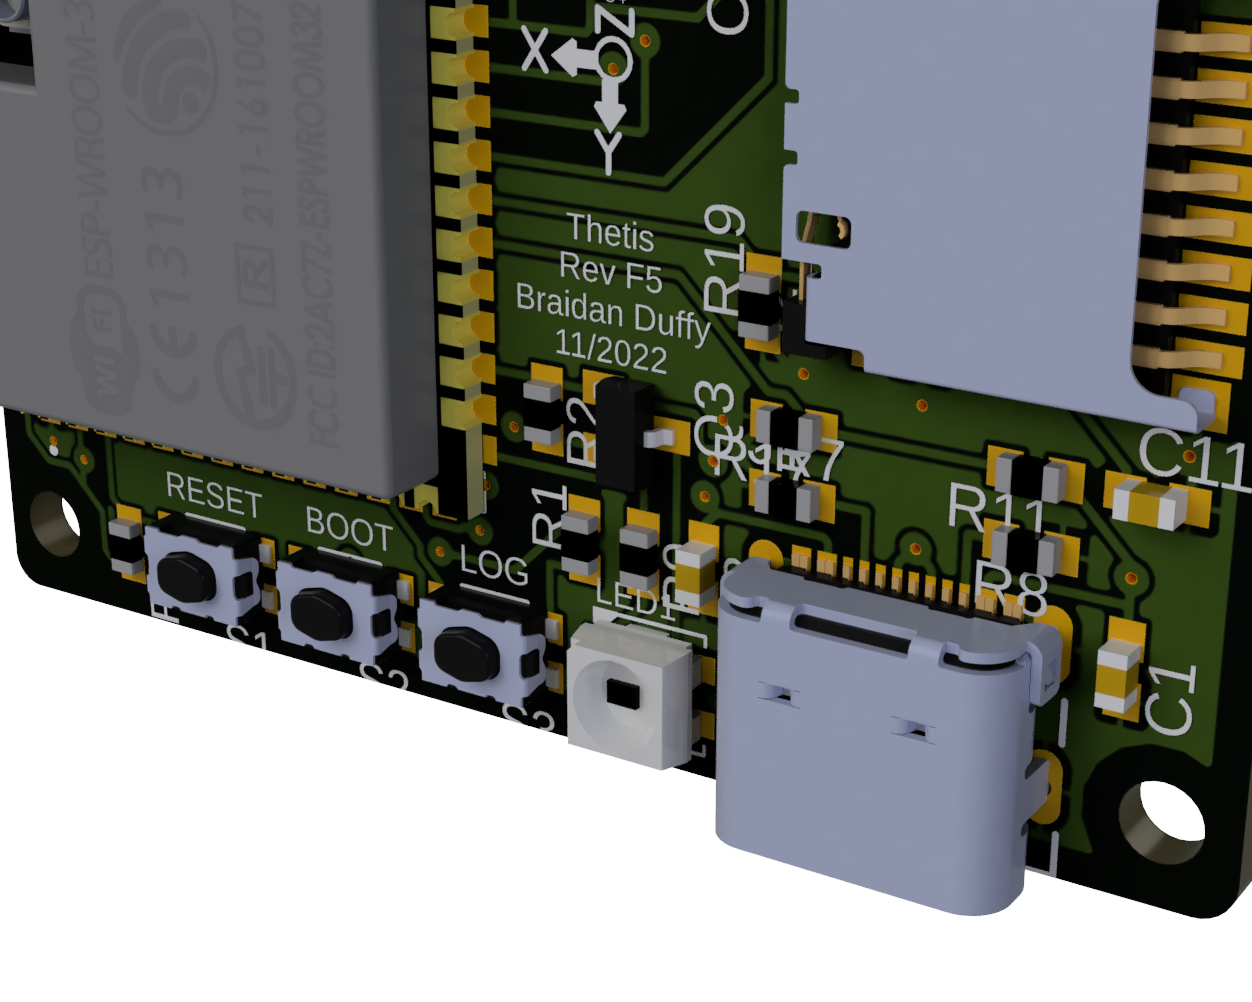
\includegraphics[width=0.3\textwidth]{LEDs/off.png} \label{subfig:error_off}}
    \caption{A blinking red and yellow \ac{LED} indicates that Thetis is switched on and in an error state according to \Fref{tab:error_codes}}
    \label{fig:error}
\end{figure}

\customTable
{l c c m{0.5\textwidth}}
{Error & Red & Yellow & Description}
{
    General & 1 & 1 & General failure state; unhandled or unknown error \\
    Settings & 1 & 2 & Board is initialized with or encounters invalid settings \\
    Low Battery & 2 & 1 & Battery voltage is below the threshold limit and the system has not automatically shutdown \\
    Battery Monitor & 2 & 2 & The battery monitoring \acs{IC} fails to initialize \\
    Temperature & 2 & 3 & The reported system temperature exceeds a threshold\tablefootnote{not currently implemented} \\
    Card Mount & 3 & 1 & The data log filesystem fails to mount to the \acs{microSD} card \\
    Card Type & 3 & 2 & The data log filesystem initializes, but reports an incorrect \acs{microSD} card type or format \\
    File Operations & 3 & 3 & A requested filesystem operation fails to execute \\
    Wi-Fi Radio & 4 & 1 & The Wi-Fi radio fails to initialize or encounters errors \\
    BlueTooth Radio & 4 & 2 & The BlueTooth radio fails to initialize or encounters errors\footnotemark[\value{footnote}] \\
    \acs{GPS} Radio & 4 & 3 & The \acs{GPS} radio fails to initialize or encounters an error \\
    \acs{IMU} & 5 & 1 & The \acs{IMU} fails to initialize or encounters an error \\
    Magnetometer & 5 & 2 & The magnetometer fails to initialize or encounters an error \\
    Fusion & 5 & 3 & The sensor fusion algorithm encounters an error\footnotemark[\value{footnote}] \\
    CANbus & 6 & 1 & The CANbus transceiver fails to initialize or encounters an error\footnotemark[\value{footnote}] \\
    Device ID & 6 & 2 & The device ID is not properly configured\footnotemark[\value{footnote}] \\
}
{Thetis error code table}
{tab:error_codes}

\subsubsection{User control}

The on-board \ac{RGB} \ac{LED} can be controlled by the user using the strobe and colour commands.  
See \Fref{sec:strobeCommand} and \Fref{sec:colourCommand} for more information.

\subsection{Secondary Diagnostic \acs{LED}}
In addition to the main \ac{RGB} \ac{LED}, Thetis also has four other monochromatic diagnostic \acp{LED} on the left and top edge of the board.
From top to bottom, these \acp{LED} are for battery charging, activity, GPS fix, and power.
Their locations are highlighted in \Fref{fig:diagnostic_led}

\ledFigure{diagnostic}{Additional monochromatic diagnostic LEDs present on Thetis}{diagnostic_led}

\begin{description}
    \item[The battery charging \ac{LED}] illuminates orange when the battery is plugged in, \ac{USB} is connected, and the battery is not at 4.2V. The board does not need to be on to charge the battery.
    \item[The activity \ac{LED}] is blue and typically only illuminated when the device is logging. This behavior can be changed in the firmware.   
    \item[The \acs{GPS} fix \ac{LED}] blinks red once per second when the GPS is acquiring a signal. Once the signal is acquired, it blinks quickly once every 15 seconds.
    \item[The power \ac{LED}] illuminates red when the 3V3 bus on the board is active; nominally when the battery or \ac{USB} is plugged in and the switch turned on.
\end{description}

    \section{Data logger}
\label{sec:dataLogger}

Thetis can function as a stand-alone data logger by streaming real-time data to a file on the \ac{microSD}.
Files created by the data logger use the .bin extension and can be downloaded from the device to be converted to \ac{CSV} files using the product software.

The data logger will create a new file in the root directory on the \ac{microSD} each time the device boots.
Files will never be overwritten or deleted by the data logger.
If the \ac{microSD} becomes full then the data logger will stop and Thetis will indicate an error.

\subsection{Start and stop}

The data logger is started or stopped by the ``Log Enable'' button (\seeSection{sec:buttons}).
As soon as the button is held for half of a second, the device will immediately begin logging.
When the operator wishes to stop logging, the ``Log Enable'' button can be held again for another half second or until the ``Activity'' LED and \acs{RGB} \acs{LED} reflect the ``Ready'' state.

\vskip 3em

\warning{The data file is not written to the microSD card filesystem until the device is commanded to stop logging.
DO NOT reset or power off the device when logging, otherwise the data may not be saved or will be corrupted!}

\subsection{File name}
\label{sec:fileName}

The file name format is ``log\textunderscore CCC.bin'' where ``CCC'' is a counter.
The counter runs between ``000'' and ``999''.
On startup, Thetis scans the microSD card and increments the counter until the next available number is encountered.
When it exceeds its maximum value, the system will throw a filesystem initialization error.
Even if the device is powered on, but does not log, a new log file will be created.
In testing environments, this may lead to multiple empty files that can obscure an actual desired data file.

\subsection{File contents}

The contents of the file is a byte stream as per the communication protocol described in \Fref{sec:communicationProtocol}.

    \section{Troubleshooting Guide}
As you use Thetis, you may encounter a variety of issues or bugs.
If the problem you encounter is not explained in Section \ref{sec:known_issues}, please create an issue in the main Thetis GitHub repository\footnote{\url{https://GitHub.com/Legohead259/Thetis-Firmware}} and explain your problem.

\subsection{Basic Diagnostics}
When you first encounter an issue with Thetis, plug it into a computer using a USB-C cable.
Turn on the device and search in your computer's device manager for the appropriate COM or Serial port for Thetis.
Use a serial terminal application like PuTTY\footnote{\url{https://putty.org/}} to open the serial port at 115200 baud rate.

\begin{figure}[H]
    \centering
    \subfloat[Thetis (green) will show up under ``Ports (COM and LPT)'' (red) in the Windows Device Manager application]{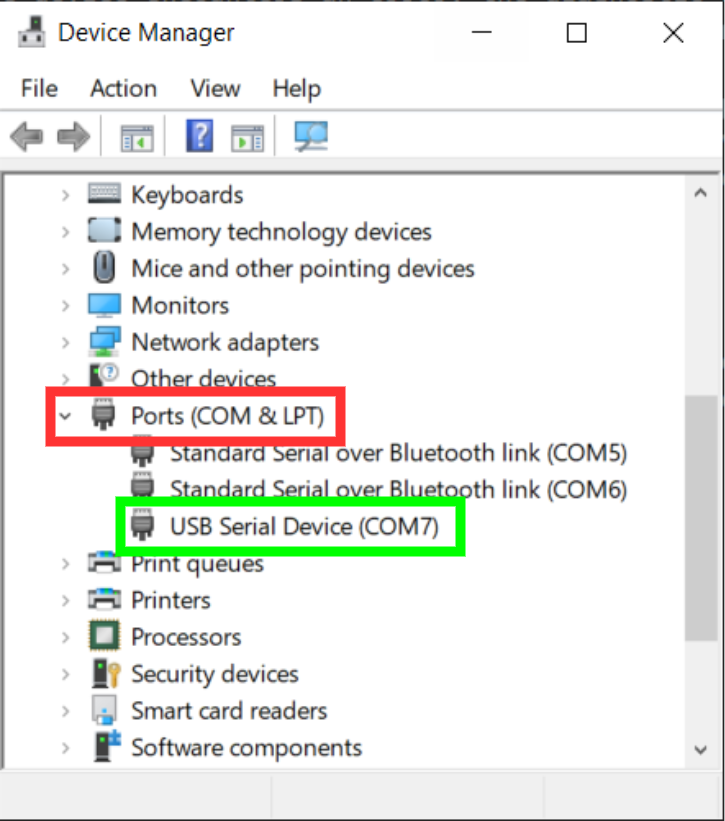
\includegraphics[width=0.45\textwidth]{troubleshooting/device_manager.png} \label{subfig:device_manager}} \hskip3ex
    \subfloat[In a serial terminal like PuTTy, enter the serial port from the device manager (green) and set the baudrate to 115200 (cyan)]{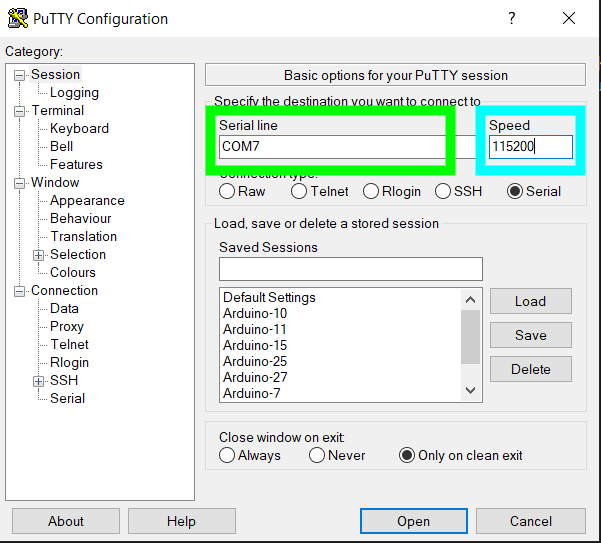
\includegraphics[width=0.45\textwidth]{troubleshooting/putty.png} \label{subfig:putty}}
    \caption{Opening the serial terminal for Thetis diagnostics}
    \label{fig:open_serial_terminal}
\end{figure}

Once the serial monitor is connected, there will be a string of data coming through.
At the start of the stream will be the diagnostic data from the initialization procedure.
The diagnostic messages are in the format: ``[Timestamp] [Log Level] Message'' where the timestamp is the current system time in ISO8601 format\footnote{yyyy-MM-ddThh:mm:ss.SSS}.
The log level is defined in \Fref{tab:log_level}.
By default, Thetis will report everything that is ``Verbose'' or below over the USB serial connection.

\customTable
{l c m{0.6\textwidth}}
{Level Name & Priority & Description}
{
    BYPASS & 0 & Indicates a message should just be passed along - only used for bypassing the typical log functions \\
    FATAL & 1 & Indicates a fatal event that cripples the device \\
    ERROR & 2 & Indicates a major error, but not fatal \\
    WARN & 3 & Indicates a substantial event that is not an error or fatal \\
    INFO & 4 & Indicates basic information for logging \\
    DEBUG & 5 & Indicates some parameter that is less important than basic information \\
    VERBOSE & 6 & Indicates some information that is less important than debug information \\
    TRACE & 7 & Information that can be used to trace down a specific bug or code execution sequence \\
}
{Log levels used by Thetis for diagnostics and their meanings}
{tab:log_level}

\begin{figure}[H]
    \centering
    \subfloat[If the device encounters an error on startup, the diagnostic log will report a ``FATAL'' event. Here, the microSD card is not present, so the filesystem fails to initialize]{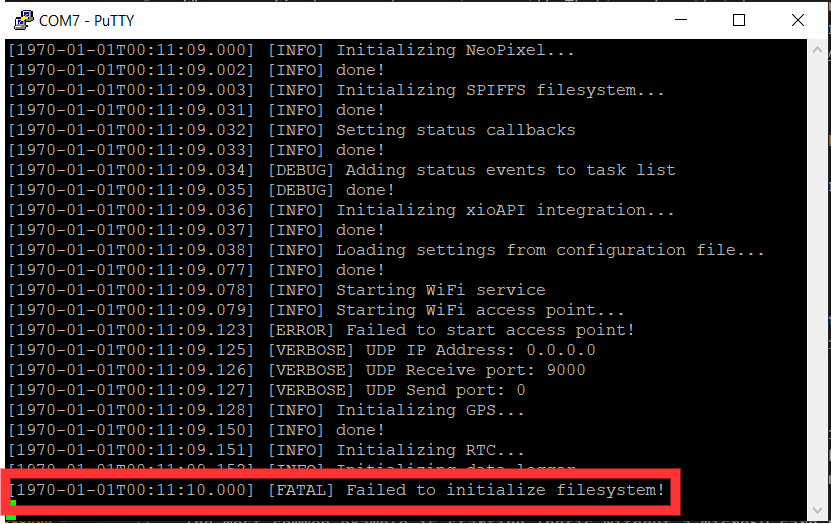
\includegraphics[width=0.45\textwidth]{troubleshooting/putty_output_error.png} \label{subfig:putty_output_error}} \hskip3ex
    \subfloat[When the device boots without error, there should be a long stream of data messages (green) after the initialization steps]{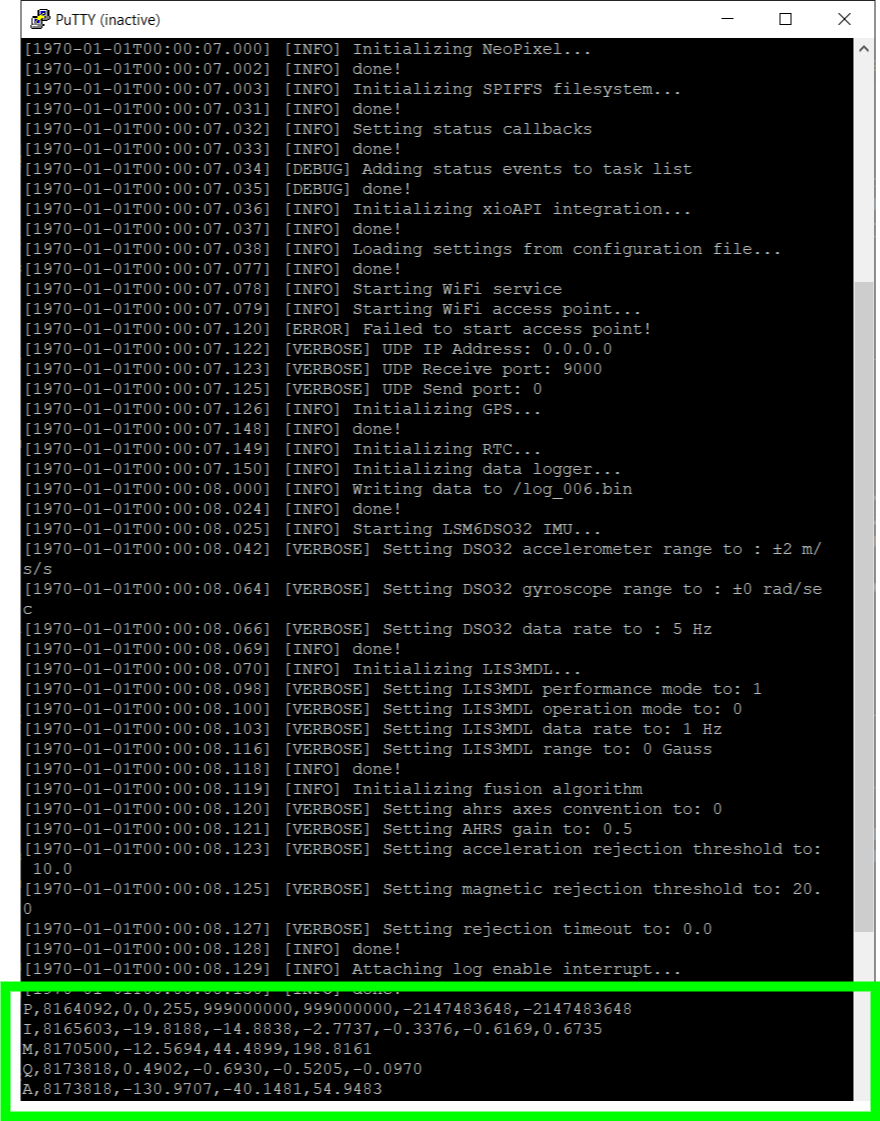
\includegraphics[width=0.45\textwidth]{troubleshooting/putty_output_good.png} \label{subfig:putty_output_good}}
    \caption{Different terminal outputs for Thetis based on error (left) or no error (right)}
    \label{fig:putty_outputs}
\end{figure}

\warning{If you are going to create a GitHub issue with your problem, it is \textbf{VERY RECOMMENDED} to include the diagnostic output from the serial monitor with your ticket. This will make diagnosing the problem easier.}

\subsection{Known Issues and Workarounds} \label{sec:known_issues}

\subsubsection{Diagnostic LED Not Working on Startup} 
When Thetis is first started, it will run through an initialization process to ensure all components are present and operating correctly.
During booting, if the device encounters an error, the diagnostic LED will not begin flashing.
The LED will remain off, but the GPS Fix and power LEDs will continue to illuminate as expected.

The most common example is starting Thetis without a microSD card present as shown in \Fref{fig:filesystem_error_bug}. 
The card is not present in the receptacle (red circle), but the device has booted without the RGB diagnostic LED illuminating any colors.
To fix this issue, place the microSD card in the receptacle and press the ``Reset'' button.
The device should start normally.

\begin{figure}[H]
    \centering
    \includegraphics[width=0.5\textwidth]{troubleshooting/filesystem_error_bug.png}
    \caption{The microSD card is not present at startup, but the device does not blink an error code.}
    \label{fig:filesystem_error_bug}
\end{figure}

\subsubsection{Thetis Not Showing Up in x-IMU3 GUI}
When Thetis is connected to a host computer over USB, it will not automatically start broadcasting data or interact with the x-IMU3 GUI.
This is because the firmware is in a diagnostic state and waiting for a serial terminal to open before streaming data.
Therefore, when using Thetis with the x-IMU3 GUI, plug it in, turn on the device and open a serial monitor to it as described above.
Then, open the x-IMU3 GUI and the device should be present.

\subsubsection{The Sensors are Reporting Data, but it is all Zeros}
Sometime
    \section{Communication protocol}
\label{sec:communicationProtocol}

All communication interfaces use the same communication protocol.
The byte stream is therefore identical for \ac{USB}, \ac{UDP}, and the files created by the data logger.
The communication protocol consists of two message types:

\begin{itemize}[nolistsep]
    \item Command messages
    \item Data messages
\end{itemize}

All messages are terminated by a \ac{LF} control character.
This termination byte will not appear anywhere else in a message and so can be used to divide a byte stream into individual messages.  
\Fref{tab:controlCharactersLFrepresentations} describes the different ways that the control character \ac{LF} may be referred to throughout this document.

\customTable
{l c c c c}
{Control character & Abbreviation & String & Hex & Decimal}
{
    \acl{LF} & \acs{LF} & \enquote{\textbackslash n} & 0x0A & 10\\
}
{Control characters \acs{LF} representations}
{tab:controlCharactersLFrepresentations}

The first byte of a message indicates the message type.
Command messages start with the character \enquote{\{} (0x7B in hex, 123 in decimal).
Data messages start with either an uppercase character or a byte value greater than 0x80 (128 in decimal) depending on the message.

\subsection{Command messages}
Command messages are sent to Thetis to read and write settings and execute commands. 
All command messages are a \ac{JSON} object containing a single key/value pair, terminated by the control character \ac{LF}.
The control character \ac{LF} must not appear anywhere else in a command message.
Thetis will acknowledge each received command message by sending a command message with the same key to the host.

The key used by command messages sent to Thetis \textbf{is case sensitive} and must be exactly as stated in the API.
For example, \enquote{serialNumber} will work, but \enquote{Serial Number} and \enquote{serial\_number} are not valid keys for a command message to read the device serial number.

\newcommand{\commandMessageExample}[2]{
    \begin{table}[H]
        \def\arraystretch{1.5}
        \begin{tabular}{l l}
            \textbf{Example:} & \texttt{\{#1\}\textbackslash n}
        \end{tabular}
    \end{table}
}

\subsubsection{Read all settings command}
The read all settings command is sent to Thetis to read all the setting values.
The key is ``readAll'' and the value is null.
See \Fref{sec:individualSettings} for a complete list of settings.  
Thetis will acknowledge a read all settings command by sending a write setting command to the host for each of its settings.

\commandMessageExample{"readAll":null}

\subsubsection{Read JSON file command}
The read JSON file command is sent to Thetis to read out the settings file stored in its non-volatile memory.
This file is a JSON file containing all the settings as key-value pairs.
See \Fref{sec:individualSettings} for a complete list of settings.
Thetis will acknowledge a read JSON file command by sending a stream reading out the entire contents of the settings file.

\commandMessageExample{"readJSON":null}

\subsubsection{Read setting command}
The read setting command is sent to Thetis to read a setting value. 
The key is the setting key and the value is null.  
See \Fref{sec:individualSettings} for a complete list of settings.  
Thetis will acknowledge a read setting command by sending a write setting command to the host.

\commandMessageExample{"serialNumber":null}

\subsubsection{Write setting command}

The write setting command is sent to Thetis to write a setting value, or sent from Thetis to the host in response to a read setting command.
The key is the setting key and the value is the setting value.
See \Fref{sec:individualSettings} for a complete list of settings.
Thetis will acknowledge a write setting command by sending a setting write command back to the host, indicating the new settings value.  
Thetis will not apply new settings until two seconds after the most recent write setting command or default command was received.

\commandMessageExample{"deviceName":"Thetis-000"}

\subsubsection{Default command}
The default command is sent to Thetis to set all settings to default values.
The key is \enquote{default} and the value is null.  
Thetis will not apply new settings until two seconds after the most recent write setting command or default command was received.

\commandMessageExample{"default":null}

\subsubsection{Apply command}

The apply command is sent to Thetis to apply all settings.  The key is \enquote{apply} and the value is null.  This command can be sent after a write setting or default command to apply settings immediately instead of after a two second delay.

\commandMessageExample{"apply":null}

\subsubsection{Save command}

The save command is sent to Thetis to save all settings to \ac{EEPROM}.  The key is \enquote{save} and the value is null.  The command acknowledgement will not be sent until the save is complete.  This may take up to 300 milliseconds.  The save command is unnecessary in most applications because Thetis will automatically save all settings on shutdown.

\commandMessageExample{"save":null}

\subsubsection{Read time command}

The read time command is sent to Thetis to read the date and time of the \ac{RTC}.  The key is \enquote{time} and the value is null.  Thetis will acknowledge a read time command by sending a write time command to the host.

\commandMessageExample{"time":null}

\subsubsection{Write time command}

The write time command is sent to Thetis to write the date and time of the \ac{RTC}, or sent from Thetis to the host in response to a read time command.  The key is \enquote{time} and the value is a string expressing the date and time in the format \enquote{YYYY-MM-DD hh:mm:ss} where each delimiter can be any non-numerical character.  Thetis will acknowledge a write time command by sending a write time command back to the host, indicating the new date and time.

\commandMessageExample{"time":"2020-01-01 00:00:00"}

\subsubsection{Ping command}

The ping command is sent to Thetis to trigger a ping response.  The key is \enquote{ping} and the value is null.  Thetis will acknowledge a ping command by sending a ping response to the host.

\commandMessageExample{"ping":null}

\subsubsection{Ping response}

The ping response is sent from Thetis to the host in response to the ping command.  The key is \enquote{ping} and the value is a \ac{JSON} object containing three key/value pairs indicating the communication interface, device name, and device serial number.  The keys are \enquote{interface}, \enquote{deviceName}, and \enquote{serialNumber}, respectively and all values are string types.

\begin{table}[H]
    \begin{tabular}{l l l}
        \textbf{Example}*\textbf{:} & \texttt{\{}\\
        & \texttt{~~"ping":~\{} &\\
        & \texttt{~~~~"interface":} & \texttt{"USB",}\\
        & \texttt{~~~~"deviceName":} & \texttt{"x-IMU3",}\\
        & \texttt{~~~~"serialNumber":} & \texttt{"0123-4567-89AB-CDEF"}\\
        & \texttt{~~\}}\\
        & \texttt{\}\textbackslash n}\\
    \end{tabular}\\
    \begin{tabular}{l}
        \\
        \footnotesize{* The actual \acs{JSON} will not include any whitespace.}
    \end{tabular}
\end{table}

\subsubsection{Reset command}

The reset command is sent to Thetis to reset Thetis.  The key is \enquote{reset} and the value is null.  A reset is equivalent to switching Thetis off and then on again.  Thetis will reset two seconds after receiving this command.

\commandMessageExample{"reset":null}

\subsubsection{Shutdown command}

The shutdown command is sent to Thetis to switch Thetis off.  The key is \enquote{shutdown} and the value is null.  Thetis will shutdown two seconds after receiving this command.

\commandMessageExample{"shutdown":null}

\subsubsection{Strobe command}
\label{sec:strobeCommand}

The strobe command is sent to Thetis to strobe the \ac{LED} bright white for 5 seconds.  The key is \enquote{strobe} and the value is null.  This command can be used to quickly locate a specific x-IMU3 when using multiple x-IMU3s.

\commandMessageExample{"strobe":null}

\subsubsection{Colour command}
\label{sec:colourCommand}

The colour command is sent to Thetis to set the \ac{LED} colour.  The key is \enquote{colour} or \enquote{color} and the value is either a \ac{RGB} hex triplet expressed as a string, or null.  Setting the colour will override the normal \ac{LED} behaviour.  A value of null will restore the normal behaviour.

\commandMessageExample{"colour":"FFFFFF"}

\subsubsection{Initialise \acs{AHRS} command}

The initialise \ac{AHRS} command is sent to Thetis to reinitialise the \ac{AHRS} algorithm.  The key is \enquote{initialise} or \enquote{initialize} and the value is null.  This command in unnecessary for normal operation and typically only used during calibration and testing.

\commandMessageExample{"initialise":null}

\subsubsection{Heading command}

The heading command is sent to Thetis to set the heading of the orientation measurement provided by the \ac{AHRS} algorithm.  The key is \enquote{heading} and the value is a number equal to the heading in degrees.  The heading command can only be used if the magnetometer is ignored in the \ac{AHRS} settings.

\commandMessageExample{"heading":0}

\subsubsection{Serial accessory command}

The serial accessory command is sent to Thetis to transmit data to a serial accessory when the serial interface is in serial accessory mode.  The key is \enquote{accessory} and the value is the data expressed as a string of up to 256 characters.  Longer strings will be truncated to the maximum size.  The string escape sequence \enquote{\textbackslash u} can be used to express any byte value as per the \ac{JSON} specification.

\commandMessageExample{"accessory":"hello \textbackslash u0077\textbackslash u006F\textbackslash u0072\textbackslash u006C\textbackslash u0064"}

\subsubsection{Note command}

The note command is sent to Thetis to generate a timestamped notification message containing a user-defined string.  The key is \enquote{note} and the value is the string of up to 127 characters.  Longer strings will be truncated to the maximum size.  This command can be used to create timestamped notes of events during data logging.

\commandMessageExample{"note":"Something happened."}

\subsubsection{Format command}

The format command is sent to Thetis to format the \ac{microSD}.  The key is \enquote{format} and the value is null.  The command acknowledgement will not be sent until the format is complete.  This will take approximately 3 seconds for an 8 GB \ac{microSD}.  Larger SD \acp{microSD} will take longer to format.  Formatting will erase all data on the SD card.

\commandMessageExample{"format":null}

\subsubsection{Self-test command}

The self-test command is sent to Thetis to perform a self-test.  The key is \enquote{test} and the value is null.  Thetis will acknowledge a self-test command by sending a self-test response to the host once the self-test is complete.  This may take up to 5 seconds.  Thetis must be stationary during the self-test.

\commandMessageExample{"test":null}

\subsubsection{Self-test response}

The self-test response is sent from Thetis to the host in response to the self-test command.  The key is \enquote{test} and the value is a \ac{JSON} object containing multiple key/value pairs.  Each key/value pair indicates the result of a test.  Each key is the test name and the value is the string "Passed" if the test was passed.

\begin{table}[H]
    \begin{tabular}{l l l}
        \textbf{Example}*\textbf{:} & \texttt{\{}\\
        & \texttt{~~"test":~\{} &\\
        & \texttt{~~~~"EEPROM":} & \texttt{"Passed",}\\
        & \texttt{~~~~"RTC":} & \texttt{"Passed",}\\
        & \texttt{~~~~"Inertial":} & \texttt{"Passed",}\\
        & \texttt{~~~~"Magnetometer":} & \texttt{"Passed",}\\
        & \texttt{~~~~"High-g Accelerometer":} & \texttt{"Passed",}\\
        & \texttt{~~~~"Battery":} & \texttt{"Passed",}\\
        & \texttt{~~~~"SD Card":} & \texttt{"Passed",}\\
        & \texttt{~~~~"Wireless":} & \texttt{"Passed",}\\
        & \texttt{~~\}}\\
        & \texttt{\}\textbackslash n}\\
    \end{tabular}\\
    \begin{tabular}{l}
        \\
        \footnotesize{* The actual \acs{JSON} will not include any whitespace.}
    \end{tabular}
\end{table}

\subsubsection{Bootloader command}

The bootloader command is sent to Thetis to put Thetis in bootloader mode.  The key is \enquote{bootloader} and the value is null.  Thetis will enter bootloader mode two seconds after receiving this command.

\commandMessageExample{"bootloader":null}

\subsubsection{Factory command}

The factory command is sent to Thetis to enable factory mode.  The key is \enquote{factory} and the value is null.  In factory mode, read-only settings can be written using the write setting command and the erase command will be enabled.

\commandMessageExample{"factory":null}

\newcommand{\commandWarning}{\warning{Incorrect use of this command may permanently damage the device.  Do not use this command unless instructed by customer support.}}

\commandWarning

\subsubsection{Erase command}

The erase command is sent to Thetis to erase the \ac{EEPROM}.  The key is \enquote{erase} and the value is null.  The command acknowledgement will not be sent until the erase is complete.  This will take approximately 700 milliseconds.  This command can only be used if factory mode is enabled.

\commandMessageExample{"erase":null}

\commandWarning

\subsection{Data messages}
\label{sec:dataMessages}

Data messages are sent from Thetis to the host to provide timestamped measurements, serial accessory data, notifications, and error messages.  Data messages will be either \ac{ASCII} or binary, depending on the device settings.

\ac{ASCII} data messages consist of multiple comma-separated values terminated by the control character character \ac{LF}.  The first value is a single uppercase character indicating the message type.  The second value is the timestamp in microseconds.  The remaining values are arguments specific to the message type.

Binary data messages are a sequence of bytes terminated by the control character \ac{LF}.  The first byte of the sequence indicates the message type.  The value of this byte is equal to 0x80 plus the first character of the equivalent \ac{ASCII} message.  The next eight bytes are the timestamp in microseconds expressed as a 64-bit unsigned integer.  The remaining bytes are arguments specific to the message type.  Numerical types use little-endian ordering.  Byte stuffing is used to remove all occurrences of the control character \ac{LF} prior to the termination byte.

\subsubsection{Byte stuffing}
\label{sec:byteStuffing}

Byte stuffing ensures that the termination byte value, 0x0A, only occurs at the end of a binary data message.  This is achieved by replacing all occurrences of the termination byte prior to termination with an escape sequence.  This process is identical to \ac{SLIP} except that the \enquote{END} byte value is defined as 0x0A.  \Fref{tab:valuesUsedByTheByteStuffingProcess} lists the values used by the byte stuffing process.

\customTable
{l l l l}
{Hex & Decimal & Name & Description}
{
0x0A & 10 & END & Message termination\\
0xDB & 219 & ESC & Message escape\\
0xDC & 220 & ESC\_END & Transposed message termination\\
0xDD & 221 & ESC\_ESC & Transposed message escape\\
}
{Values used by the byte stuffing process}
{tab:valuesUsedByTheByteStuffingProcess}

Byte stuffing is achieved by the following:

\begin{itemize}
    \item Replace each occurrence of END in the original message with the two byte sequence: ESC, ESC\_END.
    \item Replace each occurrence of ESC in the original message with the two byte sequence: ESC, ESC\_ESC.
\end{itemize}

The byte stuffing process will not modify the END that terminates the message.  \Fref{tab:byteStuffingExamples} demonstrates byte stuffing for example byte sequences terminated as binary data messages.

\begingroup
    \definecolor{colourA}{HTML}{1F77B4} % Tableau colours
    \definecolor{colourB}{HTML}{FF7F0E}
    \definecolor{colourC}{HTML}{2CA02C}
    \customTable
    {c l l}
    {Example & Before byte stuffing & After byte stuffing}
    {
    1 & \texttt{45 58 41 4D 50 4C 45 \textcolor{colourC}{0A}} & \texttt{45 58 41 4D 50 4C 45 \textcolor{colourC}{0A}}\\
    2 & \texttt{45 \textcolor{colourA}{0A} 41 4D 50 4C 45 \textcolor{colourC}{0A}} & \texttt{45 \textcolor{colourA}{DB DC} 41 4D 50 4C 45 \textcolor{colourC}{0A}}\\
    3 & \texttt{45 58 \textcolor{colourB}{DB} 4D 50 4C 45 \textcolor{colourC}{0A}} & \texttt{45 58 \textcolor{colourB}{DB DD} 4D 50 4C 45 \textcolor{colourC}{0A}}\\
    4 & \texttt{45 58 41 4D 50 \textcolor{colourB}{DB} \textcolor{colourA}{0A} \textcolor{colourC}{0A}} & \texttt{45 58 41 4D 50 \textcolor{colourB}{DB DD} \textcolor{colourA}{DB DC} \textcolor{colourC}{0A}}\\
    }
    {Byte stuffing examples}
    {tab:byteStuffingExamples}
\endgroup

\newcommand{\dataMessageTable}[2]{
    \customTable
    {c l}
    {Argument & Description}
    {
        \ifdefined\tempArgumentA 1 & \tempArgumentA\\ \fi
        \ifdefined\tempArgumentB 2 & \tempArgumentB\\ \fi
        \ifdefined\tempArgumentC 3 & \tempArgumentC\\ \fi
        \ifdefined\tempArgumentD 4 & \tempArgumentD\\ \fi
        \ifdefined\tempArgumentE 5 & \tempArgumentE\\ \fi
        \ifdefined\tempArgumentF 6 & \tempArgumentF\\ \fi
        \ifdefined\tempArgumentG 7 & \tempArgumentG\\ \fi
        \ifdefined\tempArgumentH 8 & \tempArgumentH\\ \fi
        \ifdefined\tempArgumentI 9 & \tempArgumentI\\ \fi
    }
    {#1}
    {#2}
}

\newcommand{\dataMessageExample}{
    The following message examples are for a timestamp of 1 second (1,000,000 microseconds) and argument values of:

    \definecolor{colourA}{HTML}{1F77B4} % Tableau 10 colours
    \definecolor{colourB}{HTML}{FF7F0E}
    \definecolor{colourC}{HTML}{2CA02C}
    \definecolor{colourD}{HTML}{D92728}
    \definecolor{colourE}{HTML}{9482BD}
    \definecolor{colourF}{HTML}{8C564B}
    \definecolor{colourG}{HTML}{E377C2}
    \definecolor{colourH}{HTML}{7F7F7F}
    \definecolor{colourI}{HTML}{BCBD22}
    %\definecolor{colourJ}{HTML}{17BECF}

    \begin{enumerate}[nolistsep]
        \ifdefined\tempNameA \item {\tempNameA} = \textcolor{colourA}{\tempValueA}\fi
        \ifdefined\tempNameB \item {\tempNameB} = \textcolor{colourB}{\tempValueB}\fi
        \ifdefined\tempNameC \item {\tempNameC} = \textcolor{colourC}{\tempValueC}\fi
        \ifdefined\tempNameD \item {\tempNameD} = \textcolor{colourD}{\tempValueD}\fi
        \ifdefined\tempNameE \item {\tempNameE} = \textcolor{colourE}{\tempValueE}\fi
        \ifdefined\tempNameF \item {\tempNameF} = \textcolor{colourF}{\tempValueF}\fi
        \ifdefined\tempNameG \item {\tempNameG} = \textcolor{colourG}{\tempValueG}\fi
        \ifdefined\tempNameH \item {\tempNameH} = \textcolor{colourH}{\tempValueH}\fi
        \ifdefined\tempNameI \item {\tempNameI} = \textcolor{colourI}{\tempValueI}\fi
    \end{enumerate}

    \begin{table}[H]
        \def\arraystretch{1.5}
        \begin{tabularx}{\linewidth}{l X}
            \textbf{\acs{ASCII} example:} &
            \texttt{\tempAsciiFirst,1000000}%
            \ifdefined\tempNameA \texttt{,\textcolor{colourA}{\tempAsciiA}}\fi
            \ifdefined\tempNameB \texttt{,\textcolor{colourB}{\tempAsciiB}}\fi
            \ifdefined\tempNameC \texttt{,\textcolor{colourC}{\tempAsciiC}}\fi
            \ifdefined\tempNameD \texttt{,\textcolor{colourD}{\tempAsciiD}}\fi
            \ifdefined\tempNameE \texttt{,\textcolor{colourE}{\tempAsciiE}}\fi
            \ifdefined\tempNameF \texttt{,\textcolor{colourF}{\tempAsciiF}}\fi
            \ifdefined\tempNameG \texttt{,\textcolor{colourG}{\tempAsciiG}}\fi
            \ifdefined\tempNameH \texttt{,\textcolor{colourH}{\tempAsciiH}}\fi
            \ifdefined\tempNameI \texttt{,\textcolor{colourI}{\tempAsciiI}}\fi
            \texttt{\textbackslash n}\\
            \textbf{Binary example:} &
            \texttt{{\tempBinaryFirst} 40 42 0F 00 00 00 00 00 }%
            \ifdefined\tempNameA \texttt{\textcolor{colourA}{\tempBinaryA} }\fi
            \ifdefined\tempNameB \texttt{\textcolor{colourB}{\tempBinaryB} }\fi
            \ifdefined\tempNameC \texttt{\textcolor{colourC}{\tempBinaryC} }\fi
            \ifdefined\tempNameD \texttt{\textcolor{colourD}{\tempBinaryD} }\fi
            \ifdefined\tempNameE \texttt{\textcolor{colourE}{\tempBinaryE} }\fi
            \ifdefined\tempNameF \texttt{\textcolor{colourF}{\tempBinaryF} }\fi
            \ifdefined\tempNameG \texttt{\textcolor{colourG}{\tempBinaryG} }\fi
            \ifdefined\tempNameH \texttt{\textcolor{colourH}{\tempBinaryH} }\fi
            \ifdefined\tempNameI \texttt{\textcolor{colourI}{\tempBinaryI} }\fi
            \texttt{0A}\\
        \end{tabularx}
    \end{table}
}

\subsubsection{Inertial message}

The inertial message provides timestamped gyroscope and accelerometer measurements.  Inertial messages are sent continuously at the message rate configured in the device settings.  The first value of an \ac{ASCII} message is the character \enquote{I} and the arguments are six numerical values expressed to four decimal places.  The first byte of a binary message is 0xC9 (equal to 0x80 + \enquote{I}) and the arguments are six contiguous 32-bit floats.  The message arguments are described in \Fref{tab:inertialMessageArguments}.

\begingroup
    \def\tempArgumentA{Gyroscope X axis in degrees per second}
    \def\tempArgumentB{Gyroscope Y axis in degrees per second}
    \def\tempArgumentC{Gyroscope Z axis in degrees per second}
    \def\tempArgumentD{Accelerometer X axis in g}
    \def\tempArgumentE{Accelerometer Y axis in g}
    \def\tempArgumentF{Accelerometer Z axis in g}
    \dataMessageTable
    {Inertial message arguments}
    {tab:inertialMessageArguments}
\endgroup

\begingroup
    \def\tempNameA{Gyroscope X axis}
    \def\tempNameB{Gyroscope Y axis}
    \def\tempNameC{Gyroscope Z axis}
    \def\tempNameD{Accelerometer X axis}
    \def\tempNameE{Accelerometer Y axis}
    \def\tempNameF{Accelerometer Z axis}
    \def\tempValueA{0}
    \def\tempValueB{0}
    \def\tempValueC{0}
    \def\tempValueD{0}
    \def\tempValueE{0}
    \def\tempValueF{1}
    \def\tempAsciiFirst{I}
    \def\tempAsciiA{0.0000}
    \def\tempAsciiB{0.0000}
    \def\tempAsciiC{0.0000}
    \def\tempAsciiD{0.0000}
    \def\tempAsciiE{0.0000}
    \def\tempAsciiF{1.0000}
    \def\tempBinaryFirst{C9}
    \def\tempBinaryA{00 00 00 00}
    \def\tempBinaryB{00 00 00 00}
    \def\tempBinaryC{00 00 00 00}
    \def\tempBinaryD{00 00 00 00}
    \def\tempBinaryE{00 00 00 00}
    \def\tempBinaryF{00 00 80 3F}
    \dataMessageExample
\endgroup

\subsubsection{Magnetometer message}

The magnetometer message provides timestamped magnetometer measurements.  Magnetometer messages are sent continuously at the message rate configured in the device settings.  The first value of an \ac{ASCII} message is the character \enquote{M} and the arguments are three numerical values expressed to four decimal places.  The first byte of a binary message is 0xCD (equal to 0x80 + \enquote{M}) and the arguments are three contiguous 32-bit floats.  The message arguments are described in \Fref{tab:magnetometerMessageArguments}.

\begingroup
    \def\tempArgumentA{Magnetometer X axis in \acs{a.u.}}
    \def\tempArgumentB{Magnetometer Y axis in \acs{a.u.}}
    \def\tempArgumentC{Magnetometer Z axis in \acs{a.u.}}
    \dataMessageTable
    {Magnetometer message arguments}
    {tab:magnetometerMessageArguments}
\endgroup

\begingroup
    \def\tempNameA{Magnetometer X axis}
    \def\tempNameB{Magnetometer Y axis}
    \def\tempNameC{Magnetometer Z axis}
    \def\tempValueA{1}
    \def\tempValueB{0}
    \def\tempValueC{0}
    \def\tempAsciiFirst{M}
    \def\tempAsciiA{1.0000}
    \def\tempAsciiB{0.0000}
    \def\tempAsciiC{0.0000}
    \def\tempBinaryFirst{CD}
    \def\tempBinaryA{00 00 80 3F}
    \def\tempBinaryB{00 00 00 00}
    \def\tempBinaryC{00 00 00 00}
    \dataMessageExample
\endgroup

\subsubsection{Position Message}

The position message provides timestamped \acs{GPS} data from the on-board radio.
The message are sent once per second and will only be valid or populated when the \acs{GPS} radio has a valid fix.
The first value of an \ac{ASCII} message is the character \enquote{P} and the arguments are numerical values.
The first byte of a binary message is 0xD0 (equal to 0x80 + \enquote{P}) and the arguments are several 32-bit longs and a couple 8-bit characters.
The message argument are described in \Fref{tab:positionMessageArguments}

\begingroup
    \def\tempArgumentA{GPS fix valid}
    \def\tempArgumentB{Number of satellites}
    \def\tempArgumentC{\acs{HDOP}}
    \def\tempArgumentD{Latitude in microdegrees}
    \def\tempArgumentE{Longitude in microdegrees}
    \def\tempArgumentF{Speed in meters per second}
    \def\tempArgumentG{Course in millidegrees}
    \def\tempCaption{Position message arguments}
    \def\tempLabel{tab:positionMessageArguments}
    \dataMessageTable
    {Position message arguments}
    {tab:positionMessageArguments}
\endgroup

\begingroup
    \def\tempNameA{GPS fix valid}
    \def\tempNameB{Number of satellites}
    \def\tempNameC{\acs{HDOP}}
    \def\tempNameD{Latitude}
    \def\tempNameE{Longitude}
    \def\tempNameF{Speed}
    \def\tempNameG{Course}
    \def\tempValueA{1}
    \def\tempValueB{12}
    \def\tempValueC{7}
    \def\tempValueD{280652369}
    \def\tempValueE{-806229767}
    \def\tempValueF{0}
    \def\tempValueG{0}
    \def\tempAsciiFirst{P}
    \def\tempAsciiA{1}
    \def\tempAsciiB{12}
    \def\tempAsciiC{7}
    \def\tempAsciiD{280652369}
    \def\tempAsciiE{-806229767}
    \def\tempAsciiF{0}
    \def\tempAsciiG{0}
    \def\tempBinaryFirst{50}
    \def\tempBinaryA{01}
    \def\tempBinaryB{0C}
    \def\tempBinaryC{07}
    \def\tempBinaryD{10 BA 6A 51}
    \def\tempBinaryE{30 0E 17 07}
    \def\tempBinaryF{00}
    \def\tempBinaryG{00 00 00 00}
    \dataMessageExample
\endgroup

\subsubsection{Quaternion message}

The quaternion message provides timestamped measurements of the orientation of Thetis relative to the Earth.  Quaternion messages are sent continuously at the message rate configured in the device settings.  The first value of an \ac{ASCII} message is the character \enquote{Q} and the arguments are four numerical values expressed to four decimal places.  The first byte of a binary message is 0xD1 (equal to 0x80 + \enquote{Q}) and the arguments are four contiguous 32-bit floats.  The message arguments are described in \Fref{tab:quaternionMessageArguments}.

\begingroup
    \def\tempArgumentA{Quaternion W element}
    \def\tempArgumentB{Quaternion X element}
    \def\tempArgumentC{Quaternion Y element}
    \def\tempArgumentD{Quaternion Z element}
    \def\tempCaption{Quaternion message arguments}
    \def\tempLabel{tab:quaternionMessageArguments}
    \dataMessageTable
    {Quaternion message arguments}
    {tab:quaternionMessageArguments}
\endgroup

\begingroup
    \def\tempNameA{Quaternion W element}
    \def\tempNameB{Quaternion X element}
    \def\tempNameC{Quaternion Y element}
    \def\tempNameD{Quaternion Z element}
    \def\tempValueA{1}
    \def\tempValueB{0}
    \def\tempValueC{0}
    \def\tempValueD{0}
    \def\tempAsciiFirst{Q}
    \def\tempAsciiA{1.0000}
    \def\tempAsciiB{0.0000}
    \def\tempAsciiC{0.0000}
    \def\tempAsciiD{0.0000}
    \def\tempBinaryFirst{D1}
    \def\tempBinaryA{00 00 80 3F}
    \def\tempBinaryB{00 00 00 00}
    \def\tempBinaryC{00 00 00 00}
    \def\tempBinaryD{00 00 00 00}
    \dataMessageExample
\endgroup

\subsubsection{Rotation matrix message}

The rotation matrix message provides timestamped measurements of the orientation of Thetis relative to the Earth.  Rotation matrix messages are sent continuously at the message rate configured in the device settings.  The first value of an \ac{ASCII} message is the character \enquote{R} and the arguments are nine numerical values expressed to four decimal places.  The first byte of a binary message is 0xD2 (equal to 0x80 + \enquote{R}) and the arguments are nine contiguous 32-bit floats.  The message arguments are described in \Fref{tab:rotationMatrixMessageArguments}.

\begingroup
    \def\tempArgumentA{Rotation matrix XX element}
    \def\tempArgumentB{Rotation matrix XY element}
    \def\tempArgumentC{Rotation matrix XZ element}
    \def\tempArgumentD{Rotation matrix YX element}
    \def\tempArgumentE{Rotation matrix YY element}
    \def\tempArgumentF{Rotation matrix YZ element}
    \def\tempArgumentG{Rotation matrix ZX element}
    \def\tempArgumentH{Rotation matrix ZY element}
    \def\tempArgumentI{Rotation matrix ZZ element}
    \dataMessageTable
    {Rotation matrix message arguments}
    {tab:rotationMatrixMessageArguments}
\endgroup

\begingroup
    \def\tempNameA{Rotation matrix XX element}
    \def\tempNameB{Rotation matrix XY element}
    \def\tempNameC{Rotation matrix XZ element}
    \def\tempNameD{Rotation matrix YX element}
    \def\tempNameE{Rotation matrix YY element}
    \def\tempNameF{Rotation matrix YZ element}
    \def\tempNameG{Rotation matrix ZX element}
    \def\tempNameH{Rotation matrix ZY element}
    \def\tempNameI{Rotation matrix ZZ element}
    \def\tempValueA{1}
    \def\tempValueB{0}
    \def\tempValueC{0}
    \def\tempValueD{0}
    \def\tempValueE{1}
    \def\tempValueF{0}
    \def\tempValueG{0}
    \def\tempValueH{0}
    \def\tempValueI{1}
    \def\tempAsciiFirst{R}
    \def\tempAsciiA{1.0000}
    \def\tempAsciiB{0.0000}
    \def\tempAsciiC{0.0000}
    \def\tempAsciiD{0.0000}
    \def\tempAsciiE{1.0000}
    \def\tempAsciiF{0.0000}
    \def\tempAsciiG{0.0000}
    \def\tempAsciiH{0.0000}
    \def\tempAsciiI{1.\linebreak0000} % \texttt will not line break
    \def\tempBinaryFirst{D2}
    \def\tempBinaryA{00 00 80 3F}
    \def\tempBinaryB{00 00 00 00}
    \def\tempBinaryC{00 00 00 00}
    \def\tempBinaryD{00 00 00 00}
    \def\tempBinaryE{00 00 80 3F}
    \def\tempBinaryF{00 00 00 00}
    \def\tempBinaryG{00 00 00 00}
    \def\tempBinaryH{00 00 00 00}
    \def\tempBinaryI{00 00 80 3F}
    \dataMessageExample
\endgroup

\subsubsection{Euler angles message}

The Euler angles message provides timestamped measurements of the orientation of Thetis relative to the Earth.  Euler angles messages are sent continuously at the message rate configured in the device settings.  The first value of an \ac{ASCII} message is the character \enquote{A} and the arguments are three numerical values expressed to four decimal places.  The first byte of a binary message is 0xC1 (equal to 0x80 + \enquote{A}) and the arguments are three contiguous 32-bit floats.  The message arguments are described in \Fref{tab:eulerAnglesMessageArguments}.

\begingroup
    \def\tempArgumentA{Roll angle in degrees}
    \def\tempArgumentB{Pitch angle in degrees}
    \def\tempArgumentC{Yaw angle in degrees}
    \dataMessageTable
    {Euler angles message arguments}
    {tab:eulerAnglesMessageArguments}
\endgroup

\begingroup
    \def\tempNameA{Roll angle}
    \def\tempNameB{Pitch angle}
    \def\tempNameC{Yaw angle}
    \def\tempValueA{0}
    \def\tempValueB{0}
    \def\tempValueC{0}
    \def\tempAsciiFirst{A}
    \def\tempAsciiA{0.0000}
    \def\tempAsciiB{0.0000}
    \def\tempAsciiC{0.0000}
    \def\tempBinaryFirst{C1}
    \def\tempBinaryA{00 00 00 00}
    \def\tempBinaryB{00 00 00 00}
    \def\tempBinaryC{00 00 00 00}
    \dataMessageExample
\endgroup

\subsubsection{Linear acceleration message}

The linear acceleration message provides timestamped measurements of linear acceleration and the orientation of Thetis relative to the Earth.  Linear acceleration messages are sent continuously at the message rate configured in the device settings.  The first value of an \ac{ASCII} message is the character \enquote{L} and the arguments are seven numerical values expressed to four decimal places.  The first byte of a binary message is 0xCC (equal to 0x80 + \enquote{L}) and the arguments are seven contiguous 32-bit floats.  The message arguments are described in \Fref{tab:linearAccelerationMessageArguments}.

\begingroup
    \def\tempArgumentA{Quaternion W element}
    \def\tempArgumentB{Quaternion X element}
    \def\tempArgumentC{Quaternion Y element}
    \def\tempArgumentD{Quaternion Z element}
    \def\tempArgumentE{Linear acceleration X axis in g}
    \def\tempArgumentF{Linear acceleration Y axis in g}
    \def\tempArgumentG{Linear acceleration Z axis in g}
    \def\tempCaption{Linear acceleration message arguments}
    \def\tempLabel{tab:linearAccelerationMessageArguments}
    \dataMessageTable
    {Linear acceleration message arguments}
    {tab:linearAccelerationMessageArguments}
\endgroup

\begingroup
    \def\tempNameA{Quaternion W element}
    \def\tempNameB{Quaternion X element}
    \def\tempNameC{Quaternion Y element}
    \def\tempNameD{Quaternion Z element}
    \def\tempNameE{Linear acceleration X axis}
    \def\tempNameF{Linear acceleration Y axis}
    \def\tempNameG{Linear acceleration Z axis}
    \def\tempValueA{1}
    \def\tempValueB{0}
    \def\tempValueC{0}
    \def\tempValueD{0}
    \def\tempValueE{0}
    \def\tempValueF{0}
    \def\tempValueG{0}
    \def\tempAsciiFirst{L}
    \def\tempAsciiA{1.0000}
    \def\tempAsciiB{0.0000}
    \def\tempAsciiC{0.0000}
    \def\tempAsciiD{0.0000}
    \def\tempAsciiE{0.0000}
    \def\tempAsciiF{0.0000}
    \def\tempAsciiG{0.0000}
    \def\tempBinaryFirst{CC}
    \def\tempBinaryA{00 00 80 3F}
    \def\tempBinaryB{00 00 00 00}
    \def\tempBinaryC{00 00 00 00}
    \def\tempBinaryD{00 00 00 00}
    \def\tempBinaryE{00 00 00 00}
    \def\tempBinaryF{00 00 00 00}
    \def\tempBinaryG{00 00 00 00}
    \dataMessageExample
\endgroup

\subsubsection{Earth acceleration message}

The Earth acceleration message provides timestamped measurements of Earth acceleration and the orientation of Thetis relative to the Earth.  Earth acceleration messages are sent continuously at the message rate configured in the device settings.  The first value of an \ac{ASCII} message is the character \enquote{E} and the arguments are seven numerical values expressed to four decimal places.  The first byte of a binary message is 0xC5 (equal to 0x80 + \enquote{E}) and the arguments are seven contiguous 32-bit floats.  The message arguments are described in \Fref{tab:earthAccelerationMessageArguments}.

\begingroup
    \def\tempArgumentA{Quaternion W element}
    \def\tempArgumentB{Quaternion X element}
    \def\tempArgumentC{Quaternion Y element}
    \def\tempArgumentD{Quaternion Z element}
    \def\tempArgumentE{Earth acceleration X axis in g}
    \def\tempArgumentF{Earth acceleration Y axis in g}
    \def\tempArgumentG{Earth acceleration Z axis in g}
    \def\tempCaption{Earth acceleration message arguments}
    \def\tempLabel{tab:earthAccelerationMessageArguments}
    \dataMessageTable
    {Earth acceleration message arguments}
    {tab:earthAccelerationMessageArguments}
\endgroup

\begingroup
    \def\tempNameA{Quaternion W element}
    \def\tempNameB{Quaternion X element}
    \def\tempNameC{Quaternion Y element}
    \def\tempNameD{Quaternion Z element}
    \def\tempNameE{Earth acceleration X axis}
    \def\tempNameF{Earth acceleration Y axis}
    \def\tempNameG{Earth acceleration Z axis}
    \def\tempValueA{1}
    \def\tempValueB{0}
    \def\tempValueC{0}
    \def\tempValueD{0}
    \def\tempValueE{0}
    \def\tempValueF{0}
    \def\tempValueG{0}
    \def\tempAsciiFirst{E}
    \def\tempAsciiA{1.0000}
    \def\tempAsciiB{0.0000}
    \def\tempAsciiC{0.0000}
    \def\tempAsciiD{0.0000}
    \def\tempAsciiE{0.0000}
    \def\tempAsciiF{0.0000}
    \def\tempAsciiG{0.0000}
    \def\tempBinaryFirst{C5}
    \def\tempBinaryA{00 00 80 3F}
    \def\tempBinaryB{00 00 00 00}
    \def\tempBinaryC{00 00 00 00}
    \def\tempBinaryD{00 00 00 00}
    \def\tempBinaryE{00 00 00 00}
    \def\tempBinaryF{00 00 00 00}
    \def\tempBinaryG{00 00 00 00}
    \dataMessageExample
\endgroup

\subsubsection{\acs{AHRS} status message}

The \ac{AHRS} status message provides timestamped indications of the \ac{AHRS} status flags.  An \ac{AHRS} status message is sent each time a status flag changes.  \ac{AHRS} status messages are only sent if \ac{AHRS} messages are enabled in the device settings.  The first value of an \ac{ASCII} message is the character \enquote{U} and the arguments are four numerical values expressed to four decimal places.  The first byte of a binary message is 0xD5 (equal to 0x80 + \enquote{U}) and the arguments are four contiguous 32-bit floats.  The message arguments are described in \Fref{tab:ahrsStatusnMessageArguments}.

\begingroup
    \def\tempArgumentA{Initialising}
    \def\tempArgumentB{Angular rate recovery}
    \def\tempArgumentC{Acceleration recovery}
    \def\tempArgumentD{Magnetic recovery}
    \def\tempCaption{\acs{AHRS} status message arguments}
    \def\tempLabel{tab:ahrsStatusnMessageArguments}
    \dataMessageTable
    {\acs{AHRS} status message arguments (all arguments are Boolean, see \Fref{tab:booleanArgumentValues})}
    {tab:ahrsStatusnMessageArguments}
\endgroup

\customTable
{c l}
{Value & Boolean}
{
    0 & False\\
    !0 & True\\
}
{Boolean argument values}
{tab:booleanArgumentValues}

\begingroup
    \def\tempNameA{Initialising}
    \def\tempNameB{Angular rate recovery}
    \def\tempNameC{Acceleration recovery}
    \def\tempNameD{Magnetic recovery}
    \def\tempValueA{1}
    \def\tempValueB{0}
    \def\tempValueC{0}
    \def\tempValueD{0}
    \def\tempAsciiFirst{U}
    \def\tempAsciiA{1.0000}
    \def\tempAsciiB{0.0000}
    \def\tempAsciiC{0.0000}
    \def\tempAsciiD{0.0000}
    \def\tempBinaryFirst{D5}
    \def\tempBinaryA{00 00 80 3F}
    \def\tempBinaryB{00 00 00 00}
    \def\tempBinaryC{00 00 00 00}
    \def\tempBinaryD{00 00 00 00}
    \dataMessageExample
\endgroup

\subsubsection{High-g accelerometer message}

The High-g accelerometer message provides timestamped high-g accelerometer measurements.  High-g accelerometer messages are sent continuously at the message rate configured in the device settings.  The first value of an \ac{ASCII} message is the character \enquote{H} and the arguments are three numerical values expressed to four decimal places.  The first byte of a binary message is 0xC8 (equal to 0x80 + \enquote{H}) and the arguments are three contiguous 32-bit floats.  The message arguments are described in \Fref{tab:highGMessageArguments}.

\begingroup
    \def\tempArgumentA{High-g accelerometer X axis in g}
    \def\tempArgumentB{High-g accelerometer Y axis in g}
    \def\tempArgumentC{High-g accelerometer Z axis in g}
    \dataMessageTable
    {High-g accelerometer message arguments}
    {tab:highGMessageArguments}
\endgroup

\begingroup
    \def\tempNameA{High-g accelerometer X axis}
    \def\tempNameB{High-g accelerometer Y axis}
    \def\tempNameC{High-g accelerometer Z axis}
    \def\tempValueA{0}
    \def\tempValueB{0}
    \def\tempValueC{1}
    \def\tempAsciiFirst{H}
    \def\tempAsciiA{0.0000}
    \def\tempAsciiB{0.0000}
    \def\tempAsciiC{1.0000}
    \def\tempBinaryFirst{C8}
    \def\tempBinaryA{00 00 00 00}
    \def\tempBinaryB{00 00 00 00}
    \def\tempBinaryC{00 00 80 3F}
    \dataMessageExample
\endgroup

\subsubsection{Temperature message}

The temperature message provides timestamped temperature measurements.  Temperature messages are sent continuously at the message rate configured in the device settings.  The first value of an \ac{ASCII} message is the character \enquote{T} and the argument is a numerical value expressed to four decimal places.  The first byte of a binary message is 0xD4 (equal to 0x80 + \enquote{T}) and the argument is a 32-bit float.  The message arguments are described in \Fref{tab:temperatureMessageArguments}.

\begingroup
    \def\tempArgumentA{Temperature in degrees Celsius}
    \dataMessageTable
    {Temperature message arguments}
    {tab:temperatureMessageArguments}
\endgroup

\begingroup
    \def\tempNameA{Temperature}
    \def\tempValueA{25}
    \def\tempAsciiFirst{T}
    \def\tempAsciiA{25.0000}
    \def\tempBinaryFirst{D4}
    \def\tempBinaryA{00 00 41 C8}
    \dataMessageExample
\endgroup

\subsubsection{Battery message}

The battery message message provides timestamped measurements of the battery level and charger status.  Battery message messages are sent continuously at the message rate configured in the device settings.  The first value of an \ac{ASCII} message is the character \enquote{B} and the arguments are four numerical values expressed to four decimal places.  The first byte of a binary message is 0xC2 (equal to 0x80 + \enquote{B}) and the arguments are four contiguous 32-bit floats.  The message arguments are described in \Fref{tab:batteryMessageArguments}.

\begingroup
    \def\tempArgumentA{Battery percentage}
    \def\tempArgumentB{Battery voltage in volts}
    \def\tempArgumentC{Charging status (See \Fref{tab:chargingStatusEnumeration})}
    \dataMessageTable
    {Battery message arguments}
    {tab:batteryMessageArguments}
\endgroup

\customTable
{c l}
{Charging status & Description}
{
    0 & Not connected\\
    1 & Charging\\
    2 & Charging complete\\
}
{Charging status enumeration}
{tab:chargingStatusEnumeration}

\begingroup
    \def\tempNameA{Percentage}
    \def\tempNameB{Voltage}
    \def\tempNameC{Charging status}
    \def\tempValueA{100}
    \def\tempValueB{4.2}
    \def\tempValueC{2}
    \def\tempAsciiFirst{B}
    \def\tempAsciiA{100.0000}
    \def\tempAsciiB{4.2000}
    \def\tempAsciiC{2.0000}
    \def\tempBinaryFirst{C2}
    \def\tempBinaryA{00 00 C8 42}
    \def\tempBinaryB{66 66 86 40}
    \def\tempBinaryC{00 00 00 40}
    \dataMessageExample
\endgroup

\subsubsection{\acs{RSSI} message}

The \ac{RSSI} message provides timestamped Wi-Fi \ac{RSSI} measurements.  \ac{RSSI} messages are sent continuously at the message rate configured in the device settings.  \ac{RSSI} messages will only be sent if Thetis is connected in Wi-Fi client mode.  The first value of an \ac{ASCII} message is the character \enquote{W} and the arguments are two numerical values expressed to four decimal places.  The first byte of a binary message is 0xD7 (equal to 0x80 + \enquote{W}) and the arguments are two contiguous 32-bit floats.  The message arguments are described in \Fref{tab:rssiMessageArguments}.

\begingroup
    \def\tempArgumentA{\acs{RSSI} percentage}
    \def\tempArgumentB{\acs{RSSI} power in dBm}
    \dataMessageTable
    {\acs{RSSI} message arguments}
    {tab:rssiMessageArguments}
\endgroup

\begingroup
    \def\tempNameA{\acs{RSSI} percentage}
    \def\tempNameB{\acs{RSSI} power}
    \def\tempValueA{100}
    \def\tempValueB{-50}
    \def\tempAsciiFirst{W}
    \def\tempAsciiA{100.000}
    \def\tempAsciiB{-50.0000}
    \def\tempBinaryFirst{D7}
    \def\tempBinaryA{00 00 C8 42}
    \def\tempBinaryB{00 00 48 C2}
    \dataMessageExample
\endgroup

\subsubsection{Serial accessory message}

The serial accessory message provides timestamped received serial accessory data.  Serial accessory messages are sent as serial accessory data is received as configured in the device settings.  The first value of an \ac{ASCII} message is the character \enquote{S} and the argument is the received data.  Received byte values less than 0x20 or greater than 0x7E will be replaced with the character \enquote{?} so that the argument is a string of printable characters.  The string is not null-terminated.  The first byte of a binary message is 0xD3 (equal to 0x80 + \enquote{S}) and the argument is the unmodified received data.  The message arguments are described in \Fref{tab:serialAccessoryMessageArguments}.

\begingroup
    \def\tempArgumentA{Received serial accessory data}
    \dataMessageTable
    {Serial accessory message arguments}
    {tab:serialAccessoryMessageArguments}
\endgroup

\begingroup
    \def\tempNameA{Data}
    \def\tempValueA{0x61 0x62 0x63 0x31 0x32 0x33 0xF1 0xF2 0xF3}
    \def\tempAsciiFirst{S}
    \def\tempAsciiA{abc123???}
    \def\tempBinaryFirst{D3}
    \def\tempBinaryA{61 62 63 31 32 33 F1 F2 F3}
    \dataMessageExample
\endgroup

\subsubsection{Notification message}

The notification message provides timestamped notifications of system events.  Notification messages may be sent by Thetis at any time and cannot be disabled.  The first value of an \ac{ASCII} message is the character \enquote{N}.  The first byte of a binary message is 0xCE (equal to 0x80 + \enquote{N}).  The argument of both \ac{ASCII} and binary messages is a string of printable characters.  The string is not null-terminated.  The message arguments are described in \Fref{tab:notificationMessageArguments}.

\begingroup
    \def\tempArgumentA{Notification string}
    \dataMessageTable
    {Notification message arguments}
    {tab:notificationMessageArguments}
\endgroup

\begingroup
    \def\tempNameA{String}
    \def\tempValueA{This is a notification message.}
    \def\tempAsciiFirst{N}
    \def\tempAsciiA{This is a notification message.}
    \def\tempBinaryFirst{CE}
    \def\tempBinaryA{54 68 69 73 20 69 73 20 61 20 6E 6F 74 69 66 69 63 61 74 69 6F 6E 20 6D 65 73 73 61 67 65 2E}
    \dataMessageExample
\endgroup

\subsubsection{Error message}

The error message provides timestamped notifications of errors.  Error messages may be sent by Thetis at any time and cannot be disabled.  The first value of an \ac{ASCII} message is the character \enquote{F}.  The first byte of a binary message is 0xC6 (equal to 0x80 + \enquote{F}).  The argument of both \ac{ASCII} and binary messages is a string of printable characters.  The string is not null-terminated.  The message arguments are described in \Fref{tab:errorMessageArguments}.

\begingroup
    \def\tempArgumentA{Error string}
    \dataMessageTable
    {Notification message arguments}
    {tab:errorMessageArguments}
\endgroup

\begingroup
    \def\tempNameA{String}
    \def\tempValueA{This is an error message.}
    \def\tempAsciiFirst{F}
    \def\tempAsciiA{This is an error message.}
    \def\tempBinaryFirst{C6}
    \def\tempBinaryA{54 68 69 73 20 69 73 20 61 6E 20 65 72 72 6F 72 20 6D 65 73 73 61 67 65 2E}
    \dataMessageExample
\endgroup

    \section{Sample rates, message rates, and timestamps}
\label{sec:sampleRatesMessageRatesAndTimestamps}

This section describes the relationship between sample rates and message rates, and the role of timestamps in synchronisation.

\subsection{Sample rates}

The sample rate is the rate at which measurements are sampled by a measurement source.  For example, an \ac{ADC}.  All sample rates are fixed and cannot be adjusted by the user.  Each measurement source has an independent sample clock.  The sample rate and associated data messages for each measurement source are listed in \Fref{tab:fixedSampleRatesForEachDataMessageType}.

\customTable
{l c c c}
{Measurement source & Sample rate & Sample rate error & Data messages}
{
    Inertial sensor & 400 Hz & \textpm{}0.3\% & \makecell{Inertial, Quaternion, Rotation matrix\\ Euler angles, Linear acceleration,\\ Earth acceleration, Temperature}\\
    Magnetometer & 20 Hz & \textpm{}8\% & Magnetometer\\
    High-g accelerometer & 1600 Hz & \textpm{}5\% & High-g accelerometer\\
    Battery voltage & 5 Hz & - & Battery\\
    \acs{RSSI} & 1 Hz & - & \acs{RSSI}\\
}
{Sample rate and associated data messages for each measurement source}
{tab:fixedSampleRatesForEachDataMessageType}

\subsection{Message rates}

The message rate is the rate at which a data message is sent.  The message rate of each data message type is configured by a separate message rate divisor in the device settings.  A message rate divisor is a positive integer that a fixed sample rate is divided by to obtain the message rate.  For example, if the inertial message rate divisor is 4 then the inertial message rate will be 100 messages per second.  A message rate divisor of 0 will disable the sending of that data message type.  See \Fref{sec:inertialMessageRateDivisor} to \Fref{sec:rssiMessageRateDivisor} for a detailed description and examples for each message rate divisor setting.

\subsection{Sample averaging}

If a message rate divisor is greater than 1 then the measurements in each data message will be the average of the most recent $n$ samples where $n$ equal to the message rate divisor.  The timestamp of the data message will be that of the most recent sample.  For example, if the inertial message rate divisor is 8 then the measurements in each inertial message will be the average of 8 samples and the timestamp of the message will be that of the \nth{8} sample.

\subsection{Timestamps}

The timestamp of a data message indicates the time at which a measurement was obtained.  For example, when an \ac{ADC} conversion completes.  Timestamps are therefore not affected by the sample rate error or the latency of a communication interface.  Applications that involve time-dependent calculations such as numerical integration or interpolation should not infer timing from the nominal sample rate and should instead use the timestamp of each measurement.  A timestamp is the number of microseconds since Thetis was switched on, with a resolution of one microsecond.

\subsection{Synchronisation}
\label{sec:synchronisation}

Multiple x-IMU3s operating on the same Wi-Fi network will automatically synchronise so that the timestamps from all x-IMU3s is the number of microseconds since the first x-IMU3 was switched on.  The sample clocks of synchronised x-IMU3s will remain asynchronous.  If an application requires synchronous sampling then this must be achieved in post-processing through interpolation and resampling.

    \section{Network announcement message}

The network announcement message is used by a host to discover and connect to x-IMU3s on the same network.  The message is continuously broadcast by the x-IMU3 on \ac{UDP} port 10000 at a fixed rate of one message per second.  Each message provides the device name, serial number, Wi-Fi and battery status, as well as the device settings required for a host to establish a \ac{TCP} or \ac{UDP} connection.  The message is a single \ac{JSON} object.  The key/value pairs are described in \Fref{tab:networkAnnouncementMessage}.

\customTable
{l l l}
{Key & Value type & Description}
{
    \enquote{sync} & number & Used for synchronisation\\
    \enquote{name} & string & Device name\\
    \enquote{sn} & string & Device serial number\\
    \enquote{ip} & string & x-IMU3 \acs{IP} address\\
    \enquote{port} & number & \acs{TCP} port\\
    \enquote{send} & number & \acs{UDP} send port (x-IMU3 sends to this port)\\
    \enquote{receive} & number & \acs{UDP} receive port (x-IMU3 receives on this port)\\
    \enquote{rssi} & number & \acs{RSSI} percentage (-1 in Wi-Fi AP mode)\\
    \enquote{battery} & number & Battery percentage\\
    \enquote{status} & number & Charging status (See \Fref{tab:chargingStatusEnumeration})\\
}
{Network announcement message key/value pairs}
{tab:networkAnnouncementMessage}

\begin{table}[H]
    \begin{tabular}{l l l}
        \textbf{Example}*\textbf{:} & \texttt{\{}\\
        & \texttt{~~"sync":} & \texttt{0,}\\
        & \texttt{~~"name":} & \texttt{"x-IMU3",}\\
        & \texttt{~~"sn":} & \texttt{"0123-4567-89AB-CDEF",}\\
        & \texttt{~~"ip":} & \texttt{"192.168.1.1",}\\
        & \texttt{~~"port":} & \texttt{7000,}\\
        & \texttt{~~"send":} & \texttt{8000,}\\
        & \texttt{~~"receive":} & \texttt{9000,}\\
        & \texttt{~~"rssi":} & \texttt{100,}\\
        & \texttt{~~"battery":} & \texttt{100,}\\
        & \texttt{~~"status":} & \texttt{2}\\
        & \texttt{\}}
    \end{tabular}\\
    \begin{tabular}{l}
        \\
        \footnotesize{* The actual \acs{JSON} will not include any whitespace.}
    \end{tabular}
\end{table}

    \section{Device Settings}

\subsection{Individual Settings}
\label{sec:individualSettings}

% This file was generated by individual_settings.py

\begingroup
    \def\tempSection{Calibration date (read-only)}
    \def\tempLabel{sec:calibrationDate}
    \def\tempDescription
    {
        Calibration date.
    }
    \def\tempKey{calibrationDate}
    \def\tempType{string}
    \def\tempDefault{\enquote{Unknown}}
    \deviceSetting
\endgroup

\begingroup
    \def\tempSection{System clock calibration (read-only)}
    \def\tempLabel{sec:systemClockCalibration}
    \def\tempDescription
    {
        System clock calibration.
    }
    \def\tempKey{systemClockCalibration}
    \def\tempType{number}
    \def\tempDefault{1.0}
    \deviceSetting
\endgroup

\begingroup
    \def\tempSection{\acs{RTC} calibration (read-only)}
    \def\tempLabel{sec:rtcCalibration}
    \def\tempDescription
    {
        \ac{RTC} calibration.
    }
    \def\tempKey{rtcCalibration}
    \def\tempType{number}
    \def\tempDefault{1.0}
    \deviceSetting
\endgroup

\begingroup
    \def\tempSection{Battery voltmeter sensitivity (read-only)}
    \def\tempLabel{sec:batteryVoltmeterSensitivity}
    \def\tempDescription
    {
        Battery voltmeter sensitivity.
    }
    \def\tempKey{batteryVoltmeterSensitivity}
    \def\tempType{number}
    \def\tempDefault{1.0}
    \deviceSetting
\endgroup

\begingroup
    \def\tempSection{Gyroscope misalignment (read-only)}
    \def\tempLabel{sec:gyroscopeMisalignment}
    \def\tempDescription
    {
        Gyroscope misalignment.
    }
    \def\tempKey{gyroscopeMisalignment}
    \def\tempType{array of 9 numbers}
    \def\tempDefault{[1.0, 0.0, 0.0, 0.0, 1.0, 0.0, 0.0, 0.0, 1.0]}
    \deviceSetting
\endgroup

\begingroup
    \def\tempSection{Gyroscope sensitivity (read-only)}
    \def\tempLabel{sec:gyroscopeSensitivity}
    \def\tempDescription
    {
        Gyroscope sensitivity.
    }
    \def\tempKey{gyroscopeSensitivity}
    \def\tempType{array of 3 numbers}
    \def\tempDefault{[1.0, 1.0, 1.0]}
    \deviceSetting
\endgroup

\begingroup
    \def\tempSection{Gyroscope offset (read-only)}
    \def\tempLabel{sec:gyroscopeOffset}
    \def\tempDescription
    {
        Gyroscope offset.
    }
    \def\tempKey{gyroscopeOffset}
    \def\tempType{array of 3 numbers}
    \def\tempDefault{[0.0, 0.0, 0.0]}
    \deviceSetting
\endgroup

\begingroup
    \def\tempSection{Accelerometer misalignment (read-only)}
    \def\tempLabel{sec:accelerometerMisalignment}
    \def\tempDescription
    {
        Accelerometer misalignment.
    }
    \def\tempKey{accelerometerMisalignment}
    \def\tempType{array of 9 numbers}
    \def\tempDefault{[1.0, 0.0, 0.0, 0.0, 1.0, 0.0, 0.0, 0.0, 1.0]}
    \deviceSetting
\endgroup

\begingroup
    \def\tempSection{Accelerometer sensitivity (read-only)}
    \def\tempLabel{sec:accelerometerSensitivity}
    \def\tempDescription
    {
        Accelerometer sensitivity.
    }
    \def\tempKey{accelerometerSensitivity}
    \def\tempType{array of 3 numbers}
    \def\tempDefault{[1.0, 1.0, 1.0]}
    \deviceSetting
\endgroup

\begingroup
    \def\tempSection{Accelerometer offset (read-only)}
    \def\tempLabel{sec:accelerometerOffset}
    \def\tempDescription
    {
        Accelerometer offset.
    }
    \def\tempKey{accelerometerOffset}
    \def\tempType{array of 3 numbers}
    \def\tempDefault{[0.0, 0.0, 0.0]}
    \deviceSetting
\endgroup

\begingroup
    \def\tempSection{Soft iron matrix (read-only)}
    \def\tempLabel{sec:softIronMatrix}
    \def\tempDescription
    {
        Soft iron matrix.
    }
    \def\tempKey{softIronMatrix}
    \def\tempType{array of 9 numbers}
    \def\tempDefault{[1.0, 0.0, 0.0, 0.0, 1.0, 0.0, 0.0, 0.0, 1.0]}
    \deviceSetting
\endgroup

\begingroup
    \def\tempSection{Hard iron offset (read-only)}
    \def\tempLabel{sec:hardIronOffset}
    \def\tempDescription
    {
        Hard iron offset.
    }
    \def\tempKey{hardIronOffset}
    \def\tempType{array of 3 numbers}
    \def\tempDefault{[0.0, 0.0, 0.0]}
    \deviceSetting
\endgroup

\begingroup
    \def\tempSection{High-g accelerometer misalignment (read-only)}
    \def\tempLabel{sec:highGAccelerometerMisalignment}
    \def\tempDescription
    {
        High-g accelerometer misalignment.
    }
    \def\tempKey{highGAccelerometerMisalignment}
    \def\tempType{array of 9 numbers}
    \def\tempDefault{[1.0, 0.0, 0.0, 0.0, 1.0, 0.0, 0.0, 0.0, 1.0]}
    \deviceSetting
\endgroup

\begingroup
    \def\tempSection{High-g accelerometer sensitivity (read-only)}
    \def\tempLabel{sec:highGAccelerometerSensitivity}
    \def\tempDescription
    {
        High-g accelerometer sensitivity.
    }
    \def\tempKey{highGAccelerometerSensitivity}
    \def\tempType{array of 3 numbers}
    \def\tempDefault{[1.0, 1.0, 1.0]}
    \deviceSetting
\endgroup

\begingroup
    \def\tempSection{High-g accelerometer offset (read-only)}
    \def\tempLabel{sec:highGAccelerometerOffset}
    \def\tempDescription
    {
        High-g accelerometer offset.
    }
    \def\tempKey{highGAccelerometerOffset}
    \def\tempType{array of 3 numbers}
    \def\tempDefault{[0.0, 0.0, 0.0]}
    \deviceSetting
\endgroup

\begingroup
    \def\tempSection{Device name}
    \def\tempLabel{sec:deviceName}
    \def\tempDescription
    {
        Device name.
    }
    \def\tempKey{deviceName}
    \def\tempType{string}
    \def\tempDefault{\enquote{x-IMU3}}
    \deviceSetting
\endgroup

\begingroup
    \def\tempSection{Serial number (read-only)}
    \def\tempLabel{sec:serialNumber}
    \def\tempDescription
    {
        Serial number.
    }
    \def\tempKey{serialNumber}
    \def\tempType{string}
    \def\tempDefault{\enquote{Unknown}}
    \deviceSetting
\endgroup

\begingroup
    \def\tempSection{Firmware version (read-only)}
    \def\tempLabel{sec:firmwareVersion}
    \def\tempDescription
    {
        Firmware version.
    }
    \def\tempKey{firmwareVersion}
    \def\tempType{string}
    \def\tempDefault{\enquote{Unknown}}
    \deviceSetting
\endgroup

\begingroup
    \def\tempSection{Bootloader version (read-only)}
    \def\tempLabel{sec:bootloaderVersion}
    \def\tempDescription
    {
        Bootloader version.
    }
    \def\tempKey{bootloaderVersion}
    \def\tempType{string}
    \def\tempDefault{\enquote{Unknown}}
    \deviceSetting
\endgroup

\begingroup
    \def\tempSection{Hardware version (read-only)}
    \def\tempLabel{sec:hardwareVersion}
    \def\tempDescription
    {
        Hardware version.
    }
    \def\tempKey{hardwareVersion}
    \def\tempType{string}
    \def\tempDefault{\enquote{Unknown}}
    \deviceSetting
\endgroup

\begingroup
    \def\tempSection{Serial mode}
    \def\tempLabel{sec:serialMode}
    \def\tempDescription
    {
        Serial mode.
    }
    \def\tempKey{serialMode}
    \def\tempType{number}
    \def\tempDefault{0}
    \deviceSetting
\endgroup

\begingroup
    \def\tempSection{Serial baud rate}
    \def\tempLabel{sec:serialBaudRate}
    \def\tempDescription
    {
        Serial baud rate.
    }
    \def\tempKey{serialBaudRate}
    \def\tempType{number}
    \def\tempDefault{115200}
    \deviceSetting
\endgroup

\begingroup
    \def\tempSection{Serial \acs{RTS}/\acs{CTS} enabled}
    \def\tempLabel{sec:serialRtsCtsEnabled}
    \def\tempDescription
    {
        Serial \ac{RTS}/\ac{CTS} enabled.
    }
    \def\tempKey{serialRtsCtsEnabled}
    \def\tempType{true or false}
    \def\tempDefault{false}
    \deviceSetting
\endgroup

\begingroup
    \def\tempSection{Serial accessory number of bytes}
    \def\tempLabel{sec:serialAccessoryNumberOfBytes}
    \def\tempDescription
    {
        Serial accessory number of bytes.
    }
    \def\tempKey{serialAccessoryNumberOfBytes}
    \def\tempType{number}
    \def\tempDefault{1024}
    \deviceSetting
\endgroup

\begingroup
    \def\tempSection{Serial accessory termination byte}
    \def\tempLabel{sec:serialAccessoryTerminationByte}
    \def\tempDescription
    {
        Serial accessory termination byte.
    }
    \def\tempKey{serialAccessoryTerminationByte}
    \def\tempType{number}
    \def\tempDefault{10}
    \deviceSetting
\endgroup

\begingroup
    \def\tempSection{Serial accessory timeout}
    \def\tempLabel{sec:serialAccessoryTimeout}
    \def\tempDescription
    {
        Serial accessory timeout.
    }
    \def\tempKey{serialAccessoryTimeout}
    \def\tempType{number}
    \def\tempDefault{100}
    \deviceSetting
\endgroup

\begingroup
    \def\tempSection{Wireless mode}
    \def\tempLabel{sec:wirelessMode}
    \def\tempDescription
    {
        Wireless mode.
    }
    \def\tempKey{wirelessMode}
    \def\tempType{number}
    \def\tempDefault{2}
    \deviceSetting
\endgroup

\begingroup
    \def\tempSection{Wireless firmware version (read-only)}
    \def\tempLabel{sec:wirelessFirmwareVersion}
    \def\tempDescription
    {
        Wireless firmware version.
    }
    \def\tempKey{wirelessFirmwareVersion}
    \def\tempType{string}
    \def\tempDefault{\enquote{Unknown}}
    \deviceSetting
\endgroup

\begingroup
    \def\tempSection{External antennae enabled}
    \def\tempLabel{sec:externalAntennaeEnabled}
    \def\tempDescription
    {
        External antennae enabled.
    }
    \def\tempKey{externalAntennaeEnabled}
    \def\tempType{true or false}
    \def\tempDefault{false}
    \deviceSetting
\endgroup

\begingroup
    \def\tempSection{Wi-Fi region}
    \def\tempLabel{sec:wiFiRegion}
    \def\tempDescription
    {
        Wi-Fi region.
    }
    \def\tempKey{wiFiRegion}
    \def\tempType{number}
    \def\tempDefault{2}
    \deviceSetting
\endgroup

\begingroup
    \def\tempSection{Wi-Fi \acs{MAC} address (read-only)}
    \def\tempLabel{sec:wiFiMacAddress}
    \def\tempDescription
    {
        Wi-Fi \ac{MAC} address.
    }
    \def\tempKey{wiFiMacAddress}
    \def\tempType{string}
    \def\tempDefault{0}
    \deviceSetting
\endgroup

\begingroup
    \def\tempSection{Wi-Fi \acs{IP} address (read-only)}
    \def\tempLabel{sec:wiFiIPAddress}
    \def\tempDescription
    {
        Wi-Fi \ac{IP} address.
    }
    \def\tempKey{wiFiIPAddress}
    \def\tempType{string}
    \def\tempDefault{0}
    \deviceSetting
\endgroup

\begingroup
    \def\tempSection{Wi-Fi client \acs{SSID}}
    \def\tempLabel{sec:wiFiClientSsid}
    \def\tempDescription
    {
        Wi-Fi client \ac{SSID}.
    }
    \def\tempKey{wiFiClientSsid}
    \def\tempType{string}
    \def\tempDefault{\enquote{}}
    \deviceSetting
\endgroup

\begingroup
    \def\tempSection{Wi-Fi client key}
    \def\tempLabel{sec:wiFiClientKey}
    \def\tempDescription
    {
        Wi-Fi client key.
    }
    \def\tempKey{wiFiClientKey}
    \def\tempType{string}
    \def\tempDefault{\enquote{}}
    \deviceSetting
\endgroup

\begingroup
    \def\tempSection{Wi-Fi client channel}
    \def\tempLabel{sec:wiFiClientChannel}
    \def\tempDescription
    {
        Wi-Fi client channel.
    }
    \def\tempKey{wiFiClientChannel}
    \def\tempType{number}
    \def\tempDefault{0}
    \deviceSetting
\endgroup

\begingroup
    \def\tempSection{Wi-Fi client \acs{DHCP} enabled}
    \def\tempLabel{sec:wiFiClientDhcpEnabled}
    \def\tempDescription
    {
        Wi-Fi client \ac{DHCP} enabled.
    }
    \def\tempKey{wiFiClientDhcpEnabled}
    \def\tempType{true or false}
    \def\tempDefault{true}
    \deviceSetting
\endgroup

\begingroup
    \def\tempSection{Wi-Fi client \acs{IP} address}
    \def\tempLabel{sec:wiFiClientIPAddress}
    \def\tempDescription
    {
        Wi-Fi client \ac{IP} address.
    }
    \def\tempKey{wiFiClientIPAddress}
    \def\tempType{string}
    \def\tempDefault{\enquote{192.168.1.2}}
    \deviceSetting
\endgroup

\begingroup
    \def\tempSection{Wi-Fi client netmask}
    \def\tempLabel{sec:wiFiClientNetmask}
    \def\tempDescription
    {
        Wi-Fi client netmask.
    }
    \def\tempKey{wiFiClientNetmask}
    \def\tempType{string}
    \def\tempDefault{\enquote{255.255.255.0}}
    \deviceSetting
\endgroup

\begingroup
    \def\tempSection{Wi-Fi client gateway}
    \def\tempLabel{sec:wiFiClientGateway}
    \def\tempDescription
    {
        Wi-Fi client gateway.
    }
    \def\tempKey{wiFiClientGateway}
    \def\tempType{string}
    \def\tempDefault{\enquote{192.168.1.1}}
    \deviceSetting
\endgroup

\begingroup
    \def\tempSection{Wi-Fi \acs{AP} \acs{SSID}}
    \def\tempLabel{sec:wiFiAPSsid}
    \def\tempDescription
    {
        Wi-Fi \ac{AP} \ac{SSID}.
    }
    \def\tempKey{wiFiAPSsid}
    \def\tempType{string}
    \def\tempDefault{\enquote{}}
    \deviceSetting
\endgroup

\begingroup
    \def\tempSection{Wi-Fi \acs{AP} key}
    \def\tempLabel{sec:wiFiAPKey}
    \def\tempDescription
    {
        Wi-Fi \ac{AP} key.
    }
    \def\tempKey{wiFiAPKey}
    \def\tempType{string}
    \def\tempDefault{\enquote{}}
    \deviceSetting
\endgroup

\begingroup
    \def\tempSection{Wi-Fi \acs{AP} channel}
    \def\tempLabel{sec:wiFiAPChannel}
    \def\tempDescription
    {
        Wi-Fi \ac{AP} channel.
    }
    \def\tempKey{wiFiAPChannel}
    \def\tempType{number}
    \def\tempDefault{36}
    \deviceSetting
\endgroup

\begingroup
    \def\tempSection{Wi-Fi \acs{AP} \acs{IP} address}
    \def\tempLabel{sec:wiFiAPIPAddress}
    \def\tempDescription
    {
        Wi-Fi \ac{AP} \ac{IP} address.
    }
    \def\tempKey{wiFiAPIPAddress}
    \def\tempType{string}
    \def\tempDefault{0x0101A9C0}
    \deviceSetting
\endgroup

\begingroup
    \def\tempSection{\acs{TCP} port}
    \def\tempLabel{sec:tcpPort}
    \def\tempDescription
    {
        \ac{TCP} port.
    }
    \def\tempKey{tcpPort}
    \def\tempType{number}
    \def\tempDefault{7000}
    \deviceSetting
\endgroup

\begingroup
    \def\tempSection{\acs{UDP} \acs{IP} address}
    \def\tempLabel{sec:udpIPAddress}
    \def\tempDescription
    {
        \ac{UDP} \ac{IP} address.
    }
    \def\tempKey{udpIPAddress}
    \def\tempType{string}
    \def\tempDefault{0}
    \deviceSetting
\endgroup

\begingroup
    \def\tempSection{\acs{UDP} send port}
    \def\tempLabel{sec:udpSendPort}
    \def\tempDescription
    {
        \ac{UDP} send port.
    }
    \def\tempKey{udpSendPort}
    \def\tempType{number}
    \def\tempDefault{0}
    \deviceSetting
\endgroup

\begingroup
    \def\tempSection{\acs{UDP} receive port}
    \def\tempLabel{sec:udpReceivePort}
    \def\tempDescription
    {
        \ac{UDP} receive port.
    }
    \def\tempKey{udpReceivePort}
    \def\tempType{number}
    \def\tempDefault{9000}
    \deviceSetting
\endgroup

\begingroup
    \def\tempSection{\acs{UDP} low latency}
    \def\tempLabel{sec:udpLowLatency}
    \def\tempDescription
    {
        \ac{UDP} low latency.
    }
    \def\tempKey{udpLowLatency}
    \def\tempType{true or false}
    \def\tempDefault{false}
    \deviceSetting
\endgroup

\begingroup
    \def\tempSection{Synchronisation enabled}
    \def\tempLabel{sec:synchronisationEnabled}
    \def\tempDescription
    {
        Synchronisation enabled.
    }
    \def\tempKey{synchronisationEnabled}
    \def\tempType{true or false}
    \def\tempDefault{true}
    \deviceSetting
\endgroup

\begingroup
    \def\tempSection{Synchronisation network latency}
    \def\tempLabel{sec:synchronisationNetworkLatency}
    \def\tempDescription
    {
        Synchronisation network latency.
    }
    \def\tempKey{synchronisationNetworkLatency}
    \def\tempType{number}
    \def\tempDefault{1500}
    \deviceSetting
\endgroup

\begingroup
    \def\tempSection{Bluetooth address (read-only)}
    \def\tempLabel{sec:bluetoothAddress}
    \def\tempDescription
    {
        Bluetooth address.
    }
    \def\tempKey{bluetoothAddress}
    \def\tempType{number}
    \def\tempDefault{0}
    \deviceSetting
\endgroup

\begingroup
    \def\tempSection{Bluetooth name}
    \def\tempLabel{sec:bluetoothName}
    \def\tempDescription
    {
        Bluetooth name.
    }
    \def\tempKey{bluetoothName}
    \def\tempType{string}
    \def\tempDefault{\enquote{}}
    \deviceSetting
\endgroup

\begingroup
    \def\tempSection{Bluetooth pin code}
    \def\tempLabel{sec:bluetoothPinCode}
    \def\tempDescription
    {
        Bluetooth pin code.
    }
    \def\tempKey{bluetoothPinCode}
    \def\tempType{string}
    \def\tempDefault{\enquote{}}
    \deviceSetting
\endgroup

\begingroup
    \def\tempSection{Bluetooth discovery mode}
    \def\tempLabel{sec:bluetoothDiscoveryMode}
    \def\tempDescription
    {
        Bluetooth discovery mode.
    }
    \def\tempKey{bluetoothDiscoveryMode}
    \def\tempType{number}
    \def\tempDefault{2}
    \deviceSetting
\endgroup

\begingroup
    \def\tempSection{Bluetooth paired address (read-only)}
    \def\tempLabel{sec:bluetoothPairedAddress}
    \def\tempDescription
    {
        Bluetooth paired address.
    }
    \def\tempKey{bluetoothPairedAddress}
    \def\tempType{number}
    \def\tempDefault{0}
    \deviceSetting
\endgroup

\begingroup
    \def\tempSection{Bluetooth paired link key (read-only)}
    \def\tempLabel{sec:bluetoothPairedLinkKey}
    \def\tempDescription
    {
        Bluetooth paired link key.
    }
    \def\tempKey{bluetoothPairedLinkKey}
    \def\tempType{number}
    \def\tempDefault{0}
    \deviceSetting
\endgroup

\begingroup
    \def\tempSection{Data logger enabled}
    \def\tempLabel{sec:dataLoggerEnabled}
    \def\tempDescription
    {
        Data logger enabled.
    }
    \def\tempKey{dataLoggerEnabled}
    \def\tempType{true or false}
    \def\tempDefault{false}
    \deviceSetting
\endgroup

\begingroup
    \def\tempSection{Data logger file name prefix}
    \def\tempLabel{sec:dataLoggerFileNamePrefix}
    \def\tempDescription
    {
        Data logger file name prefix.
    }
    \def\tempKey{dataLoggerFileNamePrefix}
    \def\tempType{string}
    \def\tempDefault{\enquote{}}
    \deviceSetting
\endgroup

\begingroup
    \def\tempSection{Data logger file name time enabled}
    \def\tempLabel{sec:dataLoggerFileNameTimeEnabled}
    \def\tempDescription
    {
        Data logger file name time enabled.
    }
    \def\tempKey{dataLoggerFileNameTimeEnabled}
    \def\tempType{true or false}
    \def\tempDefault{true}
    \deviceSetting
\endgroup

\begingroup
    \def\tempSection{Data logger file name counter enabled}
    \def\tempLabel{sec:dataLoggerFileNameCounterEnabled}
    \def\tempDescription
    {
        Data logger file name counter enabled.
    }
    \def\tempKey{dataLoggerFileNameCounterEnabled}
    \def\tempType{true or false}
    \def\tempDefault{false}
    \deviceSetting
\endgroup

\begingroup
    \def\tempSection{Data logger max file size}
    \def\tempLabel{sec:dataLoggerMaxFileSize}
    \def\tempDescription
    {
        Data logger max file size.
    }
    \def\tempKey{dataLoggerMaxFileSize}
    \def\tempType{number}
    \def\tempDefault{0}
    \deviceSetting
\endgroup

\begingroup
    \def\tempSection{Data logger max file period}
    \def\tempLabel{sec:dataLoggerMaxFilePeriod}
    \def\tempDescription
    {
        Data logger max file period.
    }
    \def\tempKey{dataLoggerMaxFilePeriod}
    \def\tempType{number}
    \def\tempDefault{0}
    \deviceSetting
\endgroup

\begingroup
    \def\tempSection{Axes alignment}
    \def\tempLabel{sec:axesAlignment}
    \def\tempDescription
    {
        Axes alignment.
    }
    \def\tempKey{axesAlignment}
    \def\tempType{number}
    \def\tempDefault{0}
    \deviceSetting
\endgroup

\begingroup
    \def\tempSection{Gyroscope offset correction enabled}
    \def\tempLabel{sec:gyroscopeOffsetCorrectionEnabled}
    \def\tempDescription
    {
        Gyroscope offset correction enabled.
    }
    \def\tempKey{gyroscopeOffsetCorrectionEnabled}
    \def\tempType{true or false}
    \def\tempDefault{true}
    \deviceSetting
\endgroup

\begingroup
    \def\tempSection{\acs{AHRS} axes convention}
    \def\tempLabel{sec:ahrsAxesConvention}
    \def\tempDescription
    {
        \ac{AHRS} axes convention.
    }
    \def\tempKey{ahrsAxesConvention}
    \def\tempType{number}
    \def\tempDefault{0}
    \deviceSetting
\endgroup

\begingroup
    \def\tempSection{\acs{AHRS} gain}
    \def\tempLabel{sec:ahrsGain}
    \def\tempDescription
    {
        \ac{AHRS} gain.
    }
    \def\tempKey{ahrsGain}
    \def\tempType{number}
    \def\tempDefault{0.5}
    \deviceSetting
\endgroup

\begingroup
    \def\tempSection{\acs{AHRS} ignore magnetometer}
    \def\tempLabel{sec:ahrsIgnoreMagnetometer}
    \def\tempDescription
    {
        \ac{AHRS} ignore magnetometer.
    }
    \def\tempKey{ahrsIgnoreMagnetometer}
    \def\tempType{true or false}
    \def\tempDefault{false}
    \deviceSetting
\endgroup

\begingroup
    \def\tempSection{\acs{AHRS} acceleration rejection enabled}
    \def\tempLabel{sec:ahrsAccelerationRejectionEnabled}
    \def\tempDescription
    {
        \ac{AHRS} acceleration rejection enabled.
    }
    \def\tempKey{ahrsAccelerationRejectionEnabled}
    \def\tempType{true or false}
    \def\tempDefault{true}
    \deviceSetting
\endgroup

\begingroup
    \def\tempSection{\acs{AHRS} magnetic rejection enabled}
    \def\tempLabel{sec:ahrsMagneticRejectionEnabled}
    \def\tempDescription
    {
        \ac{AHRS} magnetic rejection enabled.
    }
    \def\tempKey{ahrsMagneticRejectionEnabled}
    \def\tempType{true or false}
    \def\tempDefault{true}
    \deviceSetting
\endgroup

\begingroup
    \def\tempSection{Binary mode enabled}
    \def\tempLabel{sec:binaryModeEnabled}
    \def\tempDescription
    {
        Binary mode enabled.
    }
    \def\tempKey{binaryModeEnabled}
    \def\tempType{true or false}
    \def\tempDefault{true}
    \deviceSetting
\endgroup

\begingroup
    \def\tempSection{\acs{USB} data messages enabled}
    \def\tempLabel{sec:usbDataMessagesEnabled}
    \def\tempDescription
    {
        \ac{USB} data messages enabled.
    }
    \def\tempKey{usbDataMessagesEnabled}
    \def\tempType{true or false}
    \def\tempDefault{true}
    \deviceSetting
\endgroup

\begingroup
    \def\tempSection{Serial data messages enabled}
    \def\tempLabel{sec:serialDataMessagesEnabled}
    \def\tempDescription
    {
        Serial data messages enabled.
    }
    \def\tempKey{serialDataMessagesEnabled}
    \def\tempType{true or false}
    \def\tempDefault{true}
    \deviceSetting
\endgroup

\begingroup
    \def\tempSection{\acs{TCP} data messages enabled}
    \def\tempLabel{sec:tcpDataMessagesEnabled}
    \def\tempDescription
    {
        \ac{TCP} data messages enabled.
    }
    \def\tempKey{tcpDataMessagesEnabled}
    \def\tempType{true or false}
    \def\tempDefault{true}
    \deviceSetting
\endgroup

\begingroup
    \def\tempSection{\acs{UDP} data messages enabled}
    \def\tempLabel{sec:udpDataMessagesEnabled}
    \def\tempDescription
    {
        \ac{UDP} data messages enabled.
    }
    \def\tempKey{udpDataMessagesEnabled}
    \def\tempType{true or false}
    \def\tempDefault{true}
    \deviceSetting
\endgroup

\begingroup
    \def\tempSection{Bluetooth data messages enabled}
    \def\tempLabel{sec:bluetoothDataMessagesEnabled}
    \def\tempDescription
    {
        Bluetooth data messages enabled.
    }
    \def\tempKey{bluetoothDataMessagesEnabled}
    \def\tempType{true or false}
    \def\tempDefault{true}
    \deviceSetting
\endgroup

\begingroup
    \def\tempSection{Data logger data messages enabled}
    \def\tempLabel{sec:dataLoggerDataMessagesEnabled}
    \def\tempDescription
    {
        Data logger data messages enabled.
    }
    \def\tempKey{dataLoggerDataMessagesEnabled}
    \def\tempType{true or false}
    \def\tempDefault{true}
    \deviceSetting
\endgroup

\begingroup
    \def\tempSection{\acs{AHRS} message type}
    \def\tempLabel{sec:ahrsMessageType}
    \def\tempDescription
    {
        \ac{AHRS} message type.
    }
    \def\tempKey{ahrsMessageType}
    \def\tempType{number}
    \def\tempDefault{0}
    \deviceSetting
\endgroup

\begingroup
    \def\tempSection{Inertial message rate divisor}
    \def\tempLabel{sec:inertialMessageRateDivisor}
    \def\tempDescription
    {
        Inertial message rate divisor.
    }
    \def\tempKey{inertialMessageRateDivisor}
    \def\tempType{number}
    \def\tempDefault{8}
    \deviceSetting
\endgroup

\begingroup
    \def\tempSection{Magnetometer message rate divisor}
    \def\tempLabel{sec:magnetometerMessageRateDivisor}
    \def\tempDescription
    {
        Magnetometer message rate divisor.
    }
    \def\tempKey{magnetometerMessageRateDivisor}
    \def\tempType{number}
    \def\tempDefault{1}
    \deviceSetting
\endgroup

\begingroup
    \def\tempSection{\acs{AHRS} message rate divisor}
    \def\tempLabel{sec:ahrsMessageRateDivisor}
    \def\tempDescription
    {
        \ac{AHRS} message rate divisor.
    }
    \def\tempKey{ahrsMessageRateDivisor}
    \def\tempType{number}
    \def\tempDefault{8}
    \deviceSetting
\endgroup

\begingroup
    \def\tempSection{High-g accelerometer message rate divisor}
    \def\tempLabel{sec:highGAccelerometerMessageRateDivisor}
    \def\tempDescription
    {
        High-g accelerometer message rate divisor.
    }
    \def\tempKey{highGAccelerometerMessageRateDivisor}
    \def\tempType{number}
    \def\tempDefault{32}
    \deviceSetting
\endgroup

\begingroup
    \def\tempSection{Temperature message rate divisor}
    \def\tempLabel{sec:temperatureMessageRateDivisor}
    \def\tempDescription
    {
        Temperature message rate divisor.
    }
    \def\tempKey{temperatureMessageRateDivisor}
    \def\tempType{number}
    \def\tempDefault{5}
    \deviceSetting
\endgroup

\begingroup
    \def\tempSection{Battery message rate divisor}
    \def\tempLabel{sec:batteryMessageRateDivisor}
    \def\tempDescription
    {
        Battery message rate divisor.
    }
    \def\tempKey{batteryMessageRateDivisor}
    \def\tempType{number}
    \def\tempDefault{5}
    \deviceSetting
\endgroup

\begingroup
    \def\tempSection{\acs{RSSI} message rate divisor}
    \def\tempLabel{sec:rssiMessageRateDivisor}
    \def\tempDescription
    {
        \ac{RSSI} message rate divisor.
    }
    \def\tempKey{rssiMessageRateDivisor}
    \def\tempType{number}
    \def\tempDefault{1}
    \deviceSetting
\endgroup

\begingroup
    \def\tempSection{\acs{FTP} enabled}
    \def\tempLabel{sec:ftpEnabled}
    \def\tempDescription
    {
        \ac{FTP} enabled.
    }
    \def\tempKey{ftpEnabled}
    \def\tempType{true or false}
    \def\tempDefault{false}
    \deviceSetting
\endgroup

\begingroup
    \def\tempSection{\acs{FTP} username}
    \def\tempLabel{sec:ftpUsername}
    \def\tempDescription
    {
        \ac{FTP} username.
    }
    \def\tempKey{ftpUsername}
    \def\tempType{string}
    \def\tempDefault{\enquote{}}
    \deviceSetting
\endgroup

\begingroup
    \def\tempSection{Log print level}
    \def\tempLabel{sec:logPrintLevel}
    \def\tempDescription
    {
        Log print level.
    }
    \def\tempKey{logPrintLevel}
    \def\tempType{number}
    \def\tempDefault{0}
    \deviceSetting
\endgroup

\begingroup
    \def\tempSection{Log file level}
    \def\tempLabel{sec:logFileLevel}
    \def\tempDescription
    {
        Log file level.
    }
    \def\tempKey{logFileLevel}
    \def\tempType{number}
    \def\tempDefault{2}
    \deviceSetting
\endgroup

\begingroup
    \def\tempSection{\acs{GPS} \acs{RTC} sync enabled}
    \def\tempLabel{sec:gpsRtcSyncEnabled}
    \def\tempDescription
    {
        \ac{GPS} \ac{RTC} sync enabled.
    }
    \def\tempKey{gpsRtcSyncEnabled}
    \def\tempType{true or false}
    \def\tempDefault{false}
    \deviceSetting
\endgroup

\begingroup
    \def\tempSection{Accelerometer range}
    \def\tempLabel{sec:accelerometerRange}
    \def\tempDescription
    {
        Accelerometer range.
    }
    \def\tempKey{accelerometerRange}
    \def\tempType{number}
    \def\tempDefault{2}
    \deviceSetting
\endgroup

\begingroup
    \def\tempSection{Gyroscope range}
    \def\tempLabel{sec:gyroscopeRange}
    \def\tempDescription
    {
        Gyroscope range.
    }
    \def\tempKey{gyroscopeRange}
    \def\tempType{number}
    \def\tempDefault{0}
    \deviceSetting
\endgroup

\begingroup
    \def\tempSection{\acs{IMU} data rate}
    \def\tempLabel{sec:imuDataRate}
    \def\tempDescription
    {
        \ac{IMU} data rate.
    }
    \def\tempKey{imuDataRate}
    \def\tempType{number}
    \def\tempDefault{5}
    \deviceSetting
\endgroup

\begingroup
    \def\tempSection{Magnetometer performance mode}
    \def\tempLabel{sec:magnetometerPerformanceMode}
    \def\tempDescription
    {
        Magnetometer performance mode.
    }
    \def\tempKey{magnetometerPerformanceMode}
    \def\tempType{number}
    \def\tempDefault{1}
    \deviceSetting
\endgroup

\begingroup
    \def\tempSection{Magnetometer operation mode}
    \def\tempLabel{sec:magnetometerOperationMode}
    \def\tempDescription
    {
        Magnetometer operation mode.
    }
    \def\tempKey{magnetometerOperationMode}
    \def\tempType{number}
    \def\tempDefault{0}
    \deviceSetting
\endgroup

\begingroup
    \def\tempSection{Magnetometer data rate}
    \def\tempLabel{sec:magnetometerDataRate}
    \def\tempDescription
    {
        Magnetometer data rate.
    }
    \def\tempKey{magnetometerDataRate}
    \def\tempType{number}
    \def\tempDefault{1}
    \deviceSetting
\endgroup

\begingroup
    \def\tempSection{Magnetometer range}
    \def\tempLabel{sec:magnetometerRange}
    \def\tempDescription
    {
        Magnetometer range.
    }
    \def\tempKey{magnetometerRange}
    \def\tempType{number}
    \def\tempDefault{0}
    \deviceSetting
\endgroup

\begingroup
    \def\tempSection{Gauge reset voltage}
    \def\tempLabel{sec:gaugeResetVoltage}
    \def\tempDescription
    {
        Gauge reset voltage.
    }
    \def\tempKey{gaugeResetVoltage}
    \def\tempType{number}
    \def\tempDefault{2.5}
    \deviceSetting
\endgroup

\begingroup
    \def\tempSection{Gauge activity threshold}
    \def\tempLabel{sec:gaugeActivityThreshold}
    \def\tempDescription
    {
        Gauge activity threshold.
    }
    \def\tempKey{gaugeActivityThreshold}
    \def\tempType{number}
    \def\tempDefault{0.15}
    \deviceSetting
\endgroup

\begingroup
    \def\tempSection{Gauge hibernation threshold}
    \def\tempLabel{sec:gaugeHibernationThreshold}
    \def\tempDescription
    {
        Gauge hibernation threshold.
    }
    \def\tempKey{gaugeHibernationThreshold}
    \def\tempType{number}
    \def\tempDefault{0.1}
    \deviceSetting
\endgroup

\begingroup
    \def\tempSection{Gauge alert minimum voltage}
    \def\tempLabel{sec:gaugeAlertMinimumVoltage}
    \def\tempDescription
    {
        Gauge alert minimum voltage.
    }
    \def\tempKey{gaugeAlertMinimumVoltage}
    \def\tempType{number}
    \def\tempDefault{3.0}
    \deviceSetting
\endgroup

\begingroup
    \def\tempSection{Gauge alert maximum voltage}
    \def\tempLabel{sec:gaugeAlertMaximumVoltage}
    \def\tempDescription
    {
        Gauge alert maximum voltage.
    }
    \def\tempKey{gaugeAlertMaximumVoltage}
    \def\tempType{number}
    \def\tempDefault{4.2}
    \deviceSetting
\endgroup

\begingroup
    \def\tempSection{Fusion update rate}
    \def\tempLabel{sec:fusionUpdateRate}
    \def\tempDescription
    {
        Fusion update rate.
    }
    \def\tempKey{fusionUpdateRate}
    \def\tempType{number}
    \def\tempDefault{20}
    \deviceSetting
\endgroup



    \clearpage
    \unnumberedSection{Glossary}

\begin{acronym}
    \acro{AHRS}{Attitude Heading Reference System}
    \acro{ASCII}{American Standard Code for Information Interchange}
    \acro{CR}{Carriage Return}
    \acro{EEPROM}{Electrically Erasable Programmable Read-Only Memory}
    \acro{IMU}{Inertial Measurement Unit}
    \acro{IP}{Internet Protocol}
    \acro{JSON}{JavaScript Object Notation}
    \acro{LED}{Light-Emitting Diode}
    \acro{LF}{Line Feed}
    \acro{NVM}{Non-Volatile Memory}
    \acro{RGB}{Red Green Blue}
    \acro{RSSI}{Received Signal Strength Indicator}
    \acro{RTC}{Real-Time Clock}
    \acro{SLIP}{Serial Line Internet Protocol}
    \acro{TCP}{Transmission Control Protocol}
    \acro{UDP}{User Datagram Protocol}
    \acro{USB}{Universal Serial Bus}
    \acro{VISA}{Virtual Instrument Software Architecture}
\end{acronym}

% Examples:
% \ac{IMU} use acronym and define if first occurrence
% \acp{IMU} same as \ac but plural (adds an 's' unless \newacroplural previously defined)
% \acs{IMU} use acronym and does not define
% \acl{IMU} use definition and do not mention acronym
% \acsp{IMU} same as \acs but plural
% \acresetall resets so that all acronyms are redefined on next use


    \clearpage
    \unnumberedSection{Document version history}

\begingroup
    \def\arraystretch{1.5}
    \rowcolors{2}{gray!5}{white}
    \begin{longtable}{| >{\centering}p{.1\textwidth} | p{.2\textwidth} | >{\raggedright\arraybackslash}p{.6\textwidth} |}
        \arrayrulecolor{gray!50}\hline
        Version & Date & Changes\\
        \arrayrulecolor{gray!50}\hline
        v0.0 & April 7, 2020 &
        \begin{itemize}
            \item Advanced release
        \end{itemize}\\
        v0.1 & April 14, 2020 &
        \begin{itemize}
            \item Add overview and hardware sections
            \item Remove hyphenations
            \item Add missing acronyms to glossary
            \item Move glossary, disclaimer, and document version history to end of document
        \end{itemize}\\
        v0.2 & April 15, 2020 &
        \begin{itemize}
            \item Add missing hexadecimal notation
            \item Add linear acceleration and Earth acceleration data messages
            \item Remove pressure data message
        \end{itemize}\\
        v0.3 & April 29, 2020 &
        \begin{itemize}
            \item Add self-test commands
            \item Add technical specification section
            \item Add message rates section
            \item Add axes alignment and data message setting descriptions
        \end{itemize}\\
        v0.4 & May 20, 2020 &
        \begin{itemize}
            \item Add Wi-Fi setting descriptions
            \item Add Bluetooth as product feature
        \end{itemize}\\
        v0.5 & Jul 7, 2020 &
        \begin{itemize}
            \item Add instructions for updating x-IMU3 firmware
        \end{itemize}\\
        v0.6 & Sep 7, 2020 &
        \begin{itemize}
            \item Update board image
            \item Update technical specification
            \item Add factory and erase commands
            \item Add Sample rates, message rates, and timestamps section
        \end{itemize}\\
        v0.7 & Feb 9, 2021 &
        \begin{itemize}
            \item Add charger status enumeration
            \item Add power button section
            \item Add annotated housing image
        \end{itemize}\\
        v0.8 & Apr 15, 2021 &
        \begin{itemize}
            \item Add format command
            \item Remove result command
            \item Add colour command
            \item Add \ac{IP67} section
            \item Update Euler angles message
        \end{itemize}\\
        v0.9 & Aug 01, 2021 &
        \begin{itemize}
            \item Add C\# to overview
            \item Update board image
        \end{itemize}\\
        v0.10 & Jan 06, 2022 &
        \begin{itemize}
            \item Update device settings
            \item Add temperature technical specification
            \item Remove serial accessory rate divisor setting
            \item Add calibration section
        \end{itemize}\\
        v0.11 & Apr 06, 2022 &
        \begin{itemize}
            \item Use consistent numerical formatting in examples
            \item Add \ac{LED} section
            \item Change serial accessory command key
            \item Update battery life in overview
            \item Add data logger capacity section
            \item Use consistent terminology for high-g accelerometer
            \item Update data logger device setting keys
            \item Remove Bluetooth section
            \item Add data logger section
            \item Update network announcement message
            \item Add AHRS device settings
            \item Update images
        \end{itemize}\\
        v1.0 & Sep 26, 2022 &
        \begin{itemize}
            \item Express sensitivity as a diagonal matrix
            \item Update default clock calibration settings
            \item Update synchronisation settings
            \item Update factory command
            \item Update static accuracy
            \item Remove IP67 footnote
        \end{itemize}\\
        v1.1 & Apr 06, 2023 &
        \begin{itemize}
            \item Update network announcement message
            \item Add heading command
            \item Add axes convention setting
            \item Fix stylisation of \ac{microSD}
            \item Clarify that CR in is optional in commands messages
            \item Remove system clock and \ac{RTC} and battery voltmeter calibration
            \item Fix high-g accelerometer sample rate error
            \item Remove sentence stating that response is always in camel case
            \item Remove serial accessory transmit enabled setting
            \item Remove update device settings section
        \end{itemize}\\
        v1.2 & Jun 19, 2023 &
        \begin{itemize}
            \item Add footnote for Wi-Fi download in overview
            \item Specify accelerometer, magnetometer, and high-g accelerometer accuracy
            \item Add AHRS section to technical specification
            \item Add Ubuntu support to overview
            \item Update title page image
        \end{itemize}\\
        v1.3 & Jul 30, 2023 &
        \begin{itemize}
            \item Add Wi-Fi \ac{AP} \ac{IP} address setting
            \item Add initialise command
        \end{itemize}\\
        v1.4 & Aug 30, 2023 &
        \begin{itemize}
            \item Update device settings
            \item Remove optional CR from message termination
            \item Fix use of word \ac{microSD}
            \item Update data logger section
            \item Add mechanical section to technical specification
            \item Add static accuracy note about \acs{RMS} error
            \item Use word \enquote{x-IMU3} instead of \enquote{device}
        \end{itemize}\\
        v1.5 & Sep 07, 2023 &
        \begin{itemize}
            \item Add serial header pinout
        \end{itemize}\\
        vX.X & XXX XX, XXXX &
        \begin{itemize}
            \item Add \acs{AHRS} status data message
        \end{itemize}\\
        \arrayrulecolor{gray!50}\hline
    \end{longtable}
\endgroup


    \clearpage
    \unnumberedSection{Disclaimer}

The information in this document pertains to information related to x-io Technologies products.  This information is provided as a service to our customers, and may be used for information purposes only.

x-io Technologies assumes no liabilities or responsibilities for errors or omissions in this document.  This document may be changed at any time at x-io Technologies’s sole discretion without any prior notice to anyone.  x-io Technologies is not committed to updating this document in the future.

Copyright \textcopyright{} \the\year{} x-io Technologies.  All rights reserved.

\end{document}
